% Modified from AAAS Science LATEX template
% Use only LaTeX2e, calling the article.cls class and 12-point type.

\documentclass[11pt, a4paper, oneside]{article}
\usepackage{helvet}
\renewcommand{\familydefault}{\sfdefault}

\usepackage{graphicx}

\usepackage{indentfirst}
\setlength{\parindent}{1.5cm}

\usepackage{caption}
\captionsetup{font=small}

\usepackage{textcomp}

\usepackage{url}
\usepackage{scicite}

% Page setup

\topmargin 0.0cm
\oddsidemargin 0.2cm
\textwidth 16cm
\textheight 21cm
\footskip 1.0cm

\usepackage[legalpaper, portrait, margin=0.5in]{geometry}

\newcommand{\beginsupplement}{%
  \setcounter{table}{0}
  \renewcommand{\thetable}{S\arabic{table}}%
  \setcounter{figure}{0}
  \renewcommand{\thefigure}{S\arabic{figure}}%
}

% Abstract environment
\newenvironment{sciabstract}{%
\begin{quote} \bf}
{\end{quote}}

% Paper title
\title{
XPRESSyourself: Automating and Strengthening the High-Throughput Sequencing Toolkit
}

% Author info
\author{
% Tentative author list/order:
Jordan A. Berg,$^{1}$ Jeffrey T. Morgan,$^{1}$ Jonathan R. Belyeu,$^{2}$ Alex J. Bott,$^{1}$\\
Yeyun Ouyang,$^{1}$ Jason Gertz,$^{3}$ Aaron R. Quinlan,$^{2,4,5}$ Jared P. Rutter$^{1,6\ast}$\\
\\
\normalsize{$^{1}$Department of Biochemistry, University of Utah, Salt Lake City, UT, USA, 84112}\\
\normalsize{$^{2}$Department of Human Genetics, University of Utah, Salt Lake City, UT, USA, 84112}\\
\normalsize{$^{3}$Department of Oncological Sciences, University of Utah, Salt Lake City, UT, USA, 84112}\\
\normalsize{$^{4}$USTAR Center for Genetic Discovery, University of Utah, Salt Lake City, UT, USA, 84112}\\
\normalsize{$^{5}$Department of Biomedical Informatics, University of Utah, Salt Lake City, UT, USA, 84112}\\
\normalsize{$^{6}$Howard Hughes Medical Institute, University of Utah, Salt Lake City, UT, USA, 84112}\\
\\
\normalsize{$^\ast$To whom correspondence should be addressed; E-mail: rutter@biochem.utah.edu.}
}

% Include the date command, but leave its argument blank.
\date{}

%%%%%%%%%%%%%%%%% END OF PREAMBLE %%%%%%%%%%%%%%%%


% Initialize use of code blocks with syntax highlighting

\usepackage{listings}
\usepackage{color}

\definecolor{dkgreen}{rgb}{0,0.6,0}
\definecolor{gray}{rgb}{0.5,0.5,0.5}
\definecolor{mauve}{rgb}{0.58,0,0.82}

\lstset{frame=tb,
  language=Java,
  aboveskip=3mm,
  belowskip=3mm,
  showstringspaces=false,
  columns=flexible,
  basicstyle={\small\ttfamily},
  numbers=none,
  numberstyle=\tiny\color{gray},
  keywordstyle=\color{blue},
  commentstyle=\color{dkgreen},
  stringstyle=\color{mauve},
  breaklines=true,
  breakatwhitespace=true,
  tabsize=3
}


\begin{document}

% Double-space the manuscript.
\baselineskip24pt

% Make the title.
\maketitle



% Place your abstract within the special {sciabstract} environment.
\begin{sciabstract}
Nucleic acid sequencing is a routine and powerful tool in biological and clinical research. However, computational bottlenecks often exist for average users. XPRESSyourself is a ribosome profiling and RNA-seq analytical pipeline that aims to eliminate these barriers, standardize \textit{in silico} protocols, and decrease time-to-discovery. XPRESSyourself introduces and updates tools missing from current ribosome profiling and RNA-seq computational toolkits. Using XPRESSyourself, we were able to identify in a matter of hours putative mechanisms behind neurodegeneration during acute stress and neuroprotective mechanisms of the small molecule ISRIB using publicly available ribosome profiling data, highlighting its ability to rapidly uncover novel biological insight.
\end{sciabstract}

\section*{Keywords}
Pipeline, Ribosome Profiling, RNA-seq, Automation, Standardization, Reference Truncation

\section{Background}
High-throughput sequencing data has revolutionized biomedical, industrial, and basic science research. Specifically, RNA-seq has proven to be the forerunner technology for high quality RNA quantification within the last two decades. RNA-seq involves isolating the RNA fragments from a population of cells, incorporating these fragments into cDNA libraries, and assembling the sequenced reads to a reference genome or transcriptome to measure relative transcript abundance, differential splice variants, sequence polymorphisms, and more \cite{byron_nrg}. High-throughput sequencing technologies have been developed or adapted for a variety of technologies such as DNA sequencing, ChIP-seq, single-cell RNA-seq, and more recently, ribosome profiling \cite{ingolia_science}. \par

While vast strides have been made to implement and perfect these technologies, various bottlenecks still exist. For example, while more and more researchers are becoming accustomed to  the field of bioinformatics and computational biology, learning the intricacies of the different tools used in processing RNA-seq data can be challenging and problematic. Moreover, many users are not aware of the most up-to-date tools or the appropriate settings for their application \cite{costello_npjsba, funari_science}. Even for the experienced user, developing robust, automated pipelines that accurately process and assess quality of these datasets can be laborious. The variability that inevitably arises with each lab or bioinformatics core designing and using their own pipelines is also a significant challenge in the field. \par

While RNA-seq is a fairly matured technology, there are still an abundance of biases and idiosyncrasies associated with each analytical method or tool, of which a beginner user may not be aware. Additionally, few if any pre-existing pipelines or toolkits offer a thorough set of integrated tools for assessing common quality control metrics or reference curation, particularly in ribosome profiling. For example, a common bias in ribosome profiling libraries is a 5' and 3' read pile-up \cite{gerashchenko_nar, artieri_gr, hussman_plosg} due to longer kinetics associated with translation initiation and termination. It is therefore recommended that these regions of each transcript not be quantified when processing ribosome profiling libraries; however, no publicly available computational tools currently exist to facilitate this important step \cite{ingolia_meth, weinberg_reports}. \par

Several computational pipelines for sequencing have emerged that intend to tackle various aspects of these bottlenecks, but many suffer from usability issues, are not easily modifiable, or sacrifice quality for speed. For example, a simple internet search for RNA-seq pipelines will reveal several classes of pipelines. The first class is a tutorial labeled as a pipeline. Many instances of these can be found \cite{encode_pipeline, gdc_pipeline}; however, they are not automated, are often outdated, and can be difficult to implement. The second class is an automated pipeline, but requires extensive manual configuration \cite{pavlidis_pipeline, nfcore_pipeline, umcu_pipeline, cellgeni_pipeline}. The third class is an automated pipeline, but requires programmatic modification to change many common parameters \cite{dnanexus_pipeline, nextflow_pipeline}. Perhaps, the most user-friendly example is Galaxy, but in cases like its ribosome profiling pipeline, methods are severly outdated and a robust quality control step is lacking. In all the above cases, a thorough, robust, simple pipeline geared to the general user without sacrificing speed or quality is lacking. \par

In response to these issues surrounding the automation of sequencing technology, we built the XPRESSyourself bioinformatics suite for processing and analyzing high-throughput expression data. Architecturally, this suite is designed to work fast, while not sacrificing quality for speed. Each step of the pipeline utilizes the state of the art software package for that task, having been previously vetted by peer-reviewed benchmarking studies. Additionally, the framework that underlies the pipeline structure is designed such that updating and testing of a new module is facile for a trained bioinformatician, thus able to continuously offer the best options available to the entire community, regardless of expertise. \par

Currently, XPRESSyourself in partitioned into two main software packages. With the XPRESSpipe package, the user is provided with a complete suite of software to handle pre-processing, aligning, and quantifying of sequencing reads, performing quality control via various meta-analyses of pre- and post-processed reads. We also provide access to key quality control measures useful for assessing ribosome profiling and other RNA-seq experiments. These include read length distributions plots which are particularly helpful for ribosome profiling experiments due to the unique characteristics of the ribosome footprint-sized libraries (usually around 21-30 nt). A periodicity sub-module that tracks the P-site of ribosome footprints to assess effective capture of the characteristic 1 codon step of the ribosome. XPRESSpipe also includes a metagene analysis sub-module that shows the distribution of the relative position of all aligned reads across a representative transcript to ensure that no 5' or 3' biases occured during library preparation. As PCR duplicates can arise during library preparation, a library complexity visualization sub-module is included in the pipeline to ensure that PCR duplicates are minimized in the library and a robust population of different transcripts were captured during sequencing library preparation. The second package currently available within XPRESSyourself is XPRESSplot, which provides tools to perform the bulk of sequence analysis and generation of figures for publication, where many plot generation protocols that frequently require several hundred lines of code are condensed to a single line with minimal input from the user. XPRESSyourself suite packages are coded in Python and R, the linguae francae of computational biology and bioinformatics, allowing for easy modification and improvement by the sequencing community at large. XPRESSyourself suite packages are perpetually open source under a GPL-3.0 license at https://github.com/XPRESSyourself.


\section{Results}

\subsection{XPRESSpipe}
XPRESSpipe contains automated pipelines for ribosome profiling, single-end, and paired-end RNA-seq. The pipeline was largely designed based upon The Cancer Genome Atlas (TCGA) (https://www.cancer.gov/tcga) alignment standards and ensure standardization of read processing. In the future it is feasible that additional tunable parameters will be added. For the purposes of this manuscript, we will focus on ribosome profiling examples, while the majority of statements are also applicable to single- and paired-end RNA-seq. More details can be found in the documentation that will be continually updated as features are added, updated, or modified (https://xpresspipe.readthedocs.io/en/latest/). Table \ref{Tab:xpresspipe} outlines these parameters.

\captionof{table}{Summary of XPRESSpipe pipeline arguments.\label{Tab:xpresspipe}}
\begin{tabular}{p{5cm}p{13cm}}
 \textbf{Arguments} & \textbf{Description} \\
 \hline
 \textbf{Required} & \\
 \hline
 \texttt{-i, --input} & Path to input directory \\
 \hline
 \texttt{-o, --output} & Path to output directory \\
 \hline
 \texttt{-r, --reference} & Path to parent organism reference directory \\
 \hline
 \texttt{-g, --gtf} & Path and file name to GTF used for alignment quantification \\
 \hline
 \texttt{-e, --experiment} & Experiment name \\
 \hline
 \textbf{Optional} & \\
 \hline
 \texttt{--two\_pass} & Include option to perform a two-step alignment to map for unannotated splice-juntions \\
 \hline
 \texttt{-a, --adaptors} & Specify adaptor as string -- if ``None" is provided, software will attempt to auto-detect adaptors -- if ``POLYX" is provided as a single string in the list, polyX adaptors will be trimmed \\
 \hline
 \texttt{-q, --quality} & PHRED read quality threshold (default: 28) \\
 \hline
 \texttt{--min\_length} & Minimum read length threshold to keep for reads (default: 18) \\
 \hline
 \texttt{--deduplicate} & Include option to quantify alignment files with de-duplication \\
 \hline
 \texttt{--output\_bed} & Include option to output BED files for each aligned file \\
 \hline
 \texttt{-c, --quantification\_method} & Specify quantification method (default: Cufflinks\cite{cufflinks}) \\
 \hline
 \texttt{--feature\_type} & Specify feature type (3rd column in GFF file) to be used if quantifying with htseq (default: CDS) \\
 \hline
 \texttt{--stranded} & Specify whether library preparation was stranded (Options before || correspond with Cufflinks inputs, options after correspond with htseq inputs) \\
 \hline
 \texttt{--method} & Normalization method to perform (options: ``RPM", ``TPM", ``RPKM", ``FPKM") \\
 \hline
 \texttt{--batch} & Include path and filename of dataframe with batch normalization parameters \\
 \hline
 \texttt{--sjdbOverhang} & Sequencing platform read-length for constructing splice-aware reference previously (see STAR documentation for more information) \\
 \hline
 \texttt{--mismatchRatio} & Alignment ratio of mismatches to mapped length is less than this value (see STAR documentation for more information) \\
 \hline
 \texttt{--seedSearchStartLmax} & Adjusting this parameter by providing a lower number will improve mapping sensitivity (recommended value = 15 for reads ~ 25 nts) (see STAR documentation for more information) \\
 \hline
 \texttt{--genome\_size} & Only needs to be changed if provided argument during reference building and using a two-pass alignment \\
 \hline
 \texttt{-m, --max\_processors} & Number of max processors to use for tasks (default: No limit) \\
\end{tabular}
\newline

\subsubsection{Installation}
XPRESSpipe can be compiled from source (https://github.com/XPRESSyourself/XPRESSpipe) or a version-controlled Docker image (https://www.docker.com/) can be loaded using the following commands: \par

% Install XPRESSpipe code block
\begin{lstlisting}[language=bash, caption=Source installation., escapeinside={(*}{*)}]
# Download and unzip archived version from https://github.com/XPRESSyourself/XPRESSpipe/releases
$ cd XPRESSpipe
# Dependencies can be downloaded as follows:
$ conda env create -v -n xpresspipe -f requirements.yml
$ source activate xpresspipe # This will be executed each time you log back into the command line
# XPRESSpipe is installed as follows:
$ python setup.py install
$ echo 'export PATH="(*$\sim$*)/.local/bin:$PATH"'
\end{lstlisting}

XPRESSpipe is built upon several pre-established software packages required as dependencies. A full list can be found in the Methods. The above code block will install the required dependencies into a compartmentalized virtual environment using the Anaconda package manager. This environment will need to be activated each time XPRESSpipe is used. In order for your computer to access these installations, the locations of Anaconda and XPRESSpipe need to be accessible to the computer's list of recognized PATHs. In most cases, Anaconda should handle this automatically during installation.

When installing XPRESSpipe on a computing node, Anaconda and XPRESSpipe should be directed to the user's \texttt{$\sim$/.local/bin} directory, as follows:

% Install Anaconda code block
\begin{lstlisting}[language=bash, upquote=true, caption=Anaconda installation on compute node., escapeinside={(*}{*)}]
# Clean environment of pre-installed dependencies by admins
$ cd $HOME
$ module purge

# Get the latest anaconda2 or anaconda3 distribution and make executable
$ curl -O https://repo.anaconda.com/archive/Anaconda3-5.3.0-Linux-x86_64.sh
$ chmod 700 Anaconda3-5.3.0-Linux-x86_64.sh

# Install Anaconda in batch mode (assumes license agreed upon, setup prefix directory, and skip pre- and post- install scripts)
export INSTALL_DIR=$HOME/softwares/anaconda3/5.3.0
./Anaconda3-5.3.0-Linux-x86_64.sh -b -p $INSTALL_DIR -s

# Then perform the Source installation code block above to complete installation of XPRESSpipe, except the last step:
$ python setup.py install --prefix (*$\sim$*)/.local/bin
$ echo 'export PATH="(*$\sim$*)/.local/bin:$PATH"'
\end{lstlisting}


% Install XPRESSpipe code block
\begin{lstlisting}[language=bash, caption=Source installation on compute node., escapeinside={(*}{*)}]
# Download and unzip archived version from https://github.com/XPRESSyourself/XPRESSpipe/releases
$ cd XPRESSpipe
# Dependencies can be downloaded as follows:
$ conda env create -v -n xpresspipe -f requirements.yml # These may need to be installed manually to the user's profile depending on compute node setup
$ source activate xpresspipe # This will be executed each time you log back into the command line
# XPRESSpipe is installed as follows:
$ python setup.py install --prefix (*$\sim$*)/.local/bin
\end{lstlisting}

Docker images come with dependencies pre-installed and can be accessed as follows:

% Install XPRESSpipe code block
\begin{lstlisting}[language=bash, caption=Docker installation]
$ docker image pull jordanberg/xpresspipe:latest
\end{lstlisting}

\subsubsection{Inputs}
While inputs will vary sub-module to sub-module, and further information can be found in the documentation (https://xpresspipe.readthedocs.io/en/latest/) or by entering \texttt{xpresspipe \textless sub-module name\textgreater \ --help}, a few points of guidance are important to consider.

\begin{itemize}
\item Single-end reads should end in \texttt{.fq}, \texttt{.fastq}, or \texttt{.txt}
\item Paired-end reads should end in \texttt{.read1/2.fq} or \texttt{.r1/2.fq}, where \texttt{.fq} could also be \texttt{.fastq} or \texttt{.txt}
\item Read files can be \texttt{.zip} - or \texttt{.gz} - compressed. Decompression will be handled automatically by XPRESSpipe
\item The base transcriptome reference file should be a valid GTF file and should be named \texttt{transcripts.gtf}. We suggest using the most up-to-date Ensembl-curated GTF (https://www.ensembl.org/)
\item If specifying a group of fasta files to use for alignment or reference curation, the directory containing these files cannot contain any other files ending in \texttt{.txt} or \texttt{.fa}. It is recommended these files be given their own directory within your reference directory
\end{itemize}

\subsubsection{Reference Curation}
One of the first steps of RNA-seq alignment is curating a reference to which the alignment software will map reads. For the purposes of the current version of XPRESSpipe, a STAR \cite{star} reference should be created. An Ensembl-formatted (https://ensembl.org) GTF should also be placed in the reference directory and be named \texttt{transcripts.gtf}. Additional modifications are recommended to this file, which can be performed using this sub-module, discussed in more detail in the next section. Additionally, any chromosome \texttt{.fasta} files should be placed in their own directory within the curated reference directory. As this can be a time-consuming process, we will leave the \texttt{--max\_processors} argument as default in order to utilize all cores available to the computing unit. This entire process is handled with the \texttt{curateReference} sub-module for ease of use to the user. More on GTF modification arguments used in this code block follows in the section below.
\newline
\begin{lstlisting}[language=bash, caption=curateReference example]
$ xpresspipe curateReference -o /path/to/output/location/ \
                                -f /path/to/fasta/genome/ \
                                -g /path/transcripts.gtf \
                                --protein_coding \
                                --longest_transcript \
                                --truncate \
                                --truncate_5prime 45 \
                                --truncate_3prime 15 \
                                --sjdbOverhang 49 \
                                --max_processors None
\end{lstlisting}


\subsubsection{GTF Modification}
As ribosomal RNAs and other non-coding RNAs are highly abundant in RNA-seq experiments, it is often recommended to not include these sequences for quantification. By providing the \texttt{--protein\_coding} argument, only protein-coding genes are retained in the GTF file, which acts as a masking step of reads aligning to non-coding regions of the genome. \par

In most eukaryotes, mRNAs undergo alternative splicing. However, some quantification tools will consider the multiple annotated splice variants of a gene as a multi-mapper since they map to a location where several isoforms of the same gene overlap. These reads are either penalized or discarded. By providing the \texttt{--longest\_transcript} argument, the longest Ensembl canonical transcrtipt \cite{ensembl_canon} is retained for each gene in the GTF file. However, if using Cufflinks to quantify reads (discussed further in the next section), this is may not be recommended as Cufflinks is optimized to quantify abundances of the different isoforms of each gene \cite{cufflinks}. \par

For the purposes of ribosome profiling, where 5' and 3' transcript biases are frequent \cite{ingolia_meth, weinberg_reports}, the 5' and 3' ends of each transcript's coding space need to be trimmed to avoid quantification to this region. By providing the \texttt{--truncate} argument, the 5' and 3' ends of each transcript will be trimmed by the specified amounts. These values are set to defaults of 45 nt for 5' truncation and 15 nt for 3' truncation, as is the convention within the ribosome profiling field \cite{ingolia_meth}, but these can be modified using the \texttt{--truncate\_5prime} or \texttt{--truncate\_5prime} arguments.

\subsubsection{Read Processing}
While all intermediate steps of the pipelines can be run singly, we will describe the outline of the software in the context of the ribosome profiling pipeline. Pipelines and individual sub-modules are capable of being run in a parallel manner for each input file, thus accelerating the overall process. Descriptions of the options can be found in Table \ref{Tab:xpresspipe}.

\begin{enumerate}
  \item \textbf{Trimming}: First, reads need to be cleaned of artifacts from library creation. These include adaptors, unique molecular identifier (UMI) sequences, and technical errors in the form of low quality base calls. By doing so, non-native sequences are removed and reads can align properly to the reference. XPRESSpipe uses fastp, a faster, more accurate trimming package that has improved alignable read output \cite{fastp}. Adaptor sequence, base quality, and read length are all adjustable parameters available to the user. Additionally, features, such as UMIs can be input and used in pre-processing to remove artifacts from PCR duplication \cite{umi}.
  \item \textbf{Alignment}: After trimming, reads are then aligned to a reference genome. XPRESSpipe uses STAR, which, while being a more memory-intensive approach, is relatively fast and one of the best performing sequence alignment options currently available in regards to accuracy \cite{star, baruzzo_natmeth}. XPRESSpipe is capable of performing a single-pass, splice-aware GTF-guided alignment or a two-pass alignment of reads wherein novel splice junctions are determined and built into the reference, followed by alignment of reads to the new reference. A sorted-by-coordinate and indexed BAM file is output by STAR. We abstain from rRNA negative alignment at this step as downstream analysis of these mapped reads can be useful in comparing rRNA levels between samples to determine relative RNA degradation, or for other applications.
  \item \textbf{Post-alignment Processing}: XPRESSpipe will further process alignment files by parsing files for only unique alignments that are then passed on to the next steps. PCR duplicates are detected and marked or removed for downstream processing; however, these files are only used for revelant downstream steps (such as library complexity quality control) or if the user specifies to use these de-duplicated files in downstream steps such as read quantification. Use of de-duplicated alignment files may be advisable in situations where the library complexity profiles (discussed below) exhibit high duplication levels. However, generally the abundance of PCR-duplicates is low in properly-prepared sequencing libraries, so doing so may be overly stringent \cite{umi}. These steps are performed using samtools \cite{samtools}. Optionally, BED coverage files can also be output. These conversions are handled by bedtools \cite{bedtools}.
  \item \textbf{Read Quantification}: XPRESSpipe quantifies read alignments for each input file using Cufflinks \cite{cufflinks, count_benchmark}. Use of Cufflinks will output a read table with normalized counts as well as a counts table for downstream applications where required. If masking of non-coding RNAs is desired, a \texttt{protein\_coding} modified GTF file should be provided for the \texttt{--gtf} argument. Optionally, the user can use HTSeq with the \texttt{intersection-nonempty} method as default \cite{htseq, count_benchmark}. Our rationale for including this quantification method is that it conforms to current default TCGA standards and may still be useful in some applications. When using HTSeq, it is important to provide the longest-transcript only GTF to avoid counting a read mapping across multiple isoforms of the same gene as a multimapper. Because of limitations such as this, we recommend usage of Cufflinks at this step. However, HTSeq is recommended if processing ribosome profiling data as it allows selection of feature type across which to quantify, thus allowing for quantification across the CDS instead of exon.
  \item \textbf{Normalization}: Methods for count normalization are available within XPRESSpipe by way of the XPRESSplot package described later. For normalizations involving transcript length, the appropriate GTF must be provided. Current sample normalization methods available include reads-per-million (RPM), Reads-per-kilobase-million (RPKM) or Fragments-per-kilobase-million (FPKM), and transcripts per million (TPM) normalization \cite{evans_briefbio}. For samples sequenced on different flow cells, prepared by different individuals, or on different days, the \texttt{--batch} argument should be provided along with the appropriate metadata matrix, which is then processed by way of XPRESSplot using the ComBat package \cite{sva}.
  \item \textbf{Quality Control}:
  An important step in RNA-seq analysis is proper quality control of sequencing samples to ensure the interpreted downstream results are reliable. XPRESSpipe performs a variety of quality control measures. For each analysis type, high-resolution, publication quality summary figures are output for all samples in a given experiment for quick reference to the user.

    \begin{itemize}
      \item \textbf{Read Length Distribution}: Per sample, the lengths of all reads are analyzed by FastQC \cite{fastqc} after trimming. By assessing the read distribution of each sample, the user can ensure the expected read size was sequenced. This is particularly helpful in ribosome profiling experiments for verifying the requisite 21-30 nt ribosome footprints were inserted into the sequencing library successfully \cite{ingolia_meth}. Metrics are compiled and plotted by XPRESSpipe.

      \item \textbf{Library Complexity}: Measuring library complexity is an effective method for analyzing the robustness of a sequencing experiment in capturing various, unique RNA species. As the majority of RNA-seq preparation methods involve a PCR step, at times certain fragments are favored and over-amplified in contrast to others. By plotting the number of PCR replicates versus expression level for each gene, one can determine how successful the library preparation was at reducing these biases and at capturing a robust population of different RNA species. This analysis is performed using dupRadar \cite{dupradar} where inputs are PCR duplicate-tagged BAM files output by XPRESSpipe by way of samtools \cite{samtools}. Metrics are then compiled and plotted by XPRESSpipe.

      \item \textbf{Metagene Estimation Profile}: In order to identify any general 5' or 3' transcript biases in captured reads, a metagene profile can be created for each sample. This is performed by determining the meta-genomic coordinate for each aligned read in exon space. Required inputs are an indexed BAM file and an unmodified GTF reference file and outputs are metagene metrics, individual plots, and summary plots.

      \item \textbf{Codon Phasing/Periodicity Estimation Profile}: In ribosome profiling, a useful measure of a successful experiment comes by investigating the codon phasing of ribosome footprints \cite{ingolia_meth}. To do so, the P-site is calculated for each mapped ribosome footprint by taking the genomic coordinate 16 nucleotides upstream of the 3' end of each transcript falling within the acceptable range of ribosome footprints and measuring the distance in nucleotides along CDS space to the start codon from this coordinate \cite{ribowaltz}. The same inputs are required as for the \texttt{metagene} sub-module. This method is intended as a quality control and will provide a good estimate of codon phasing in ribosome profiling data. However, it does forgo any further normalization, therefore it may not be best suited for more in-depth studies of codon phasing dynamics.

      \item \textbf{rRNA Depletion Probe}: Ribosomal RNA (rRNA) contamination is common in RNA-seq library preparation and the bulk of RNA in a cell at any given time is dedicated to rRNA. As unique rRNA sequences are relatively few, sequencing of these reads becomes highly repetative and often biologically uninteresting in the context of transcription. Depletion of these sequences is often desired in order to have better depth of coverage of mRNA sequences. In order to facilitate this depletion, many commercial kits are available that target specific rRNA sequences for depletion, or that enrich for mRNA polyA tails. However, and especially in the case of ribosome profiling experiments, where RNA is digested by an RNase to create ribosome footprints, many commercial depletion kits will not perform sufficiently and polyA selection kits are inoperable as footprints will not have the requisite polyA sequence. To this end, custom rRNA probes are recommended \cite{ingolia_meth, ingolia_science}. \texttt{rrnaProbe} will analyze the over-represented sequences between footprint libraries after adaptor and quality trimming and compile conserved k-mers across the overall experiment and output a rank ordered list of these sequences for probe design.

    \end{itemize}
\end{enumerate}


\subsubsection{Outputs}
While outputs will vary sub-module to sub-module, generally, the user will specify a parent output directory and necessary sub-directories will be created based on the step in the pipeline. Further information can be found in the documentation (https://xpresspipe.readthedocs.io/en/latest/) or by entering \texttt{xpresspipe \textless sub-module name\textgreater \ --help} in the command line. Figure \ref{fig:outputs} provides an example of the output file scheme for XPRESSpipe. For a complete pipeline run, the user can expect BAM alignment files, a collated count table of all samples in the experiment, and quality control figures and metrics. For almost all sub-modules, a log file will also be output to summarize user options provided, track performance, and report errors.

\begin{figure}
\centering
  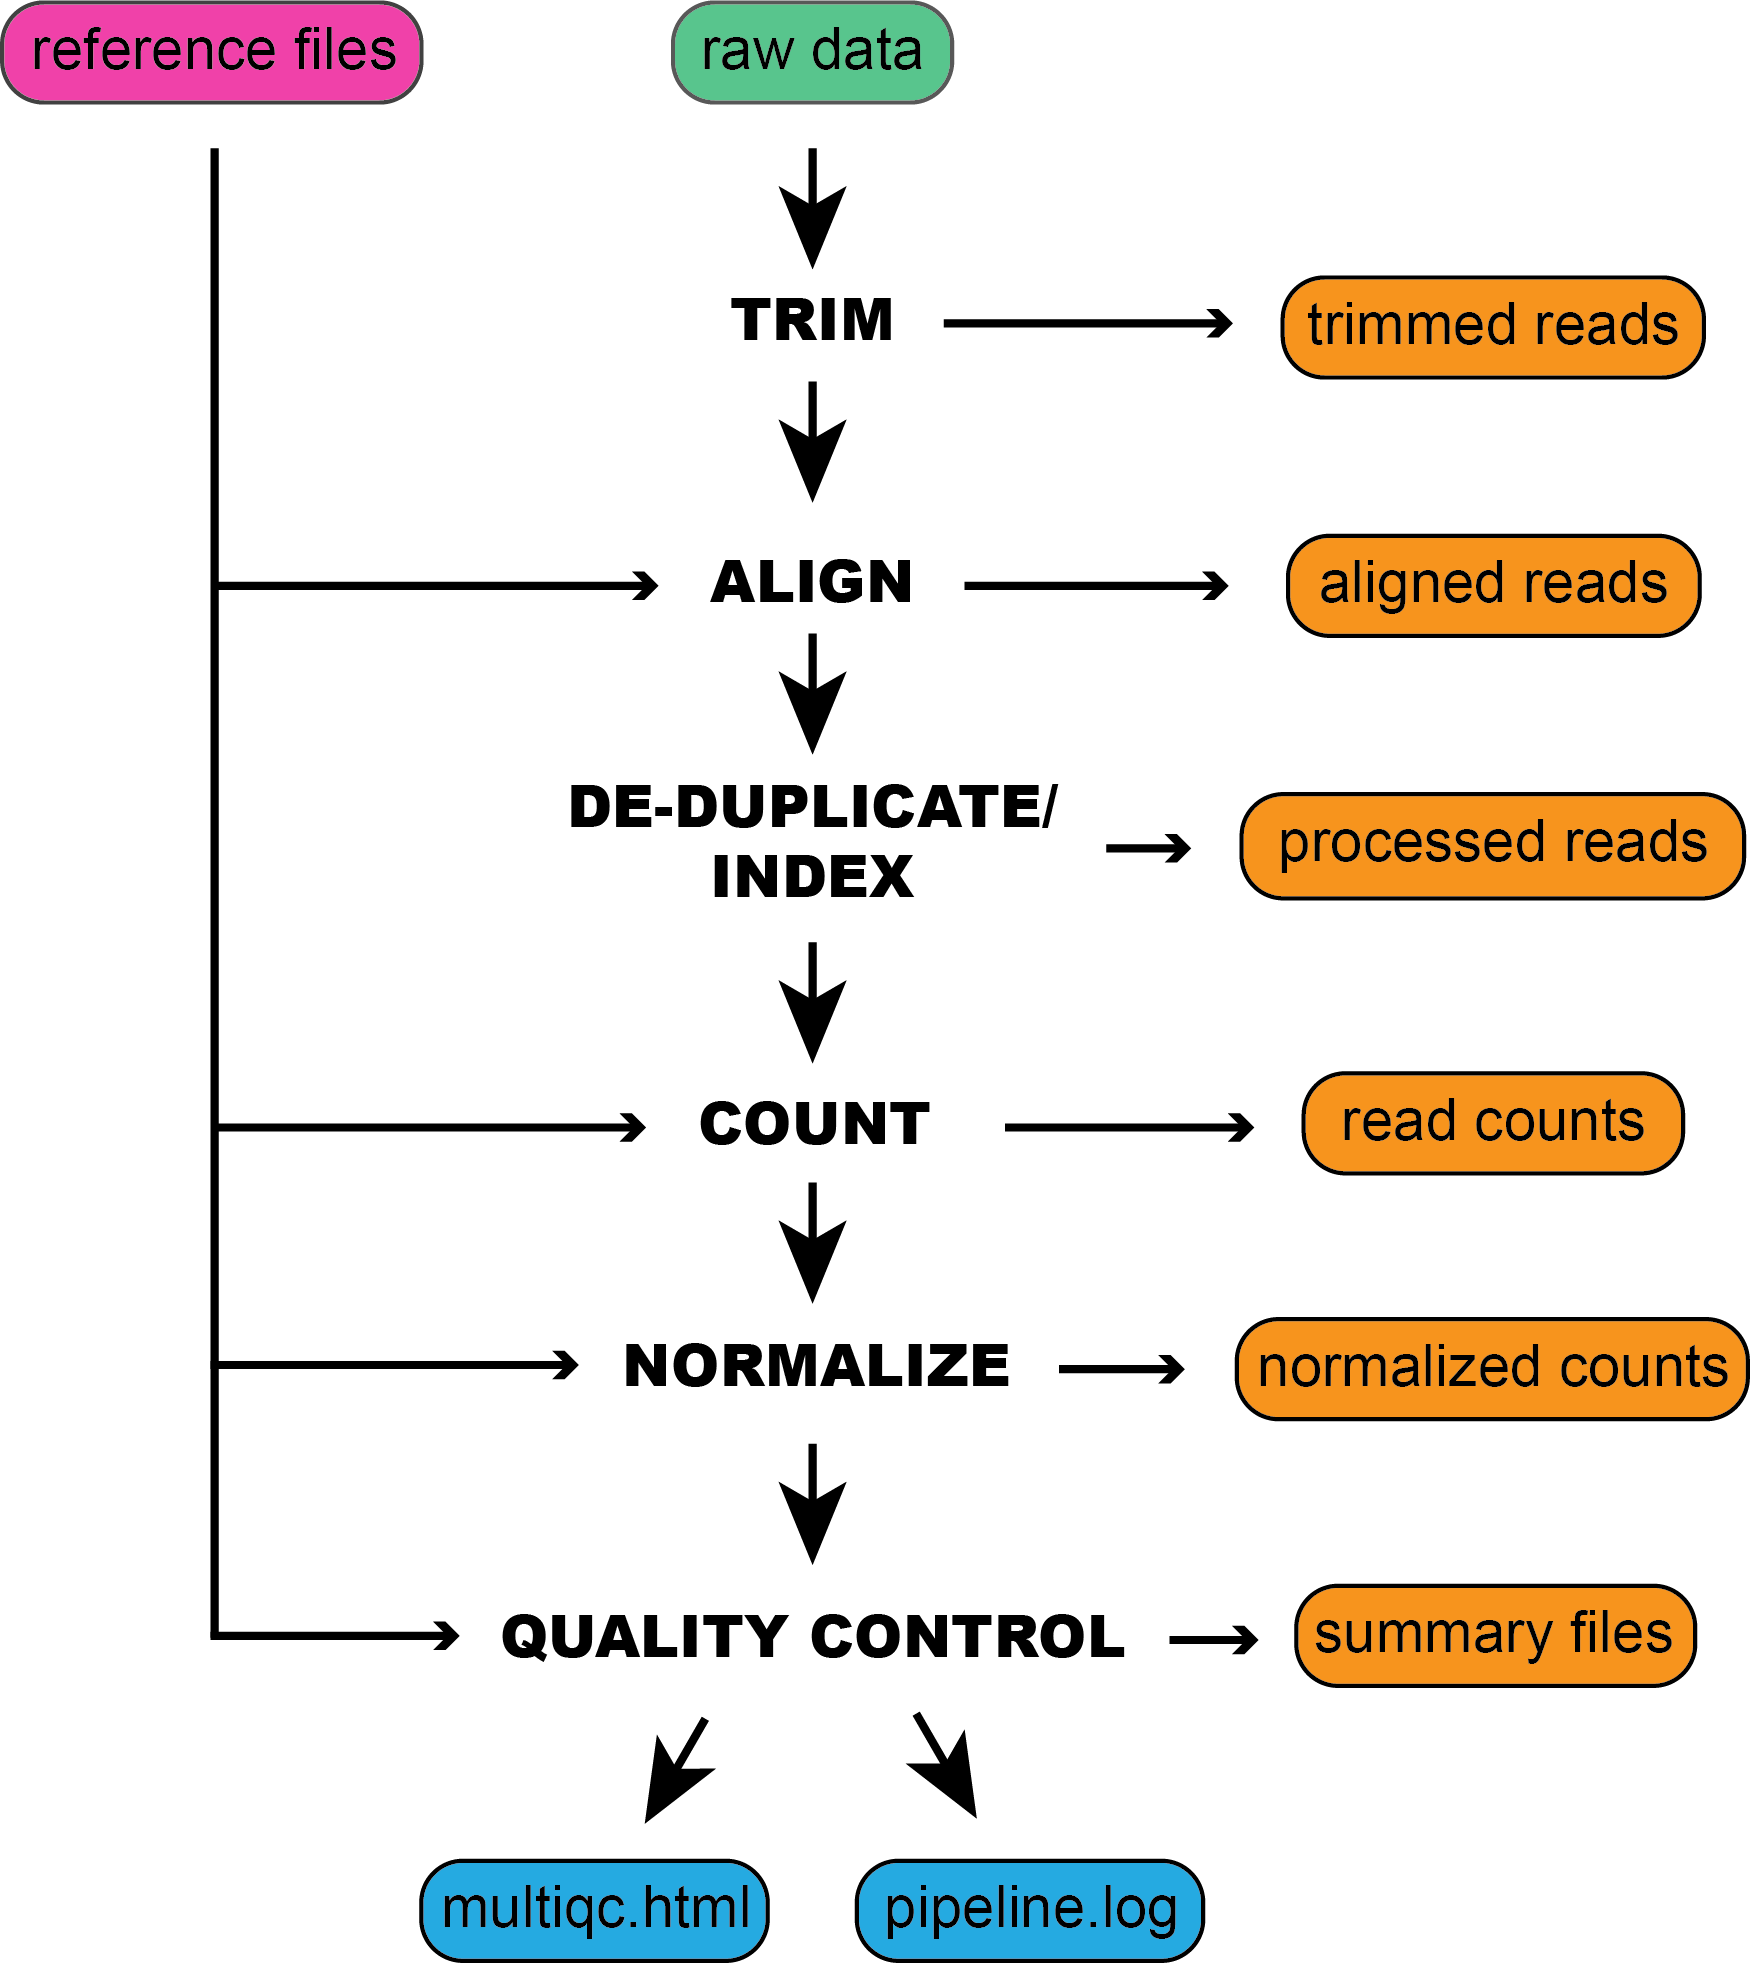
\includegraphics[width=120mm]{figures/xpresspipe_overview.png}
  \caption{An example schematic of the inputs required by XPRESSpipe and organization of the ouputs.}
  \label{fig:outputs}
\end{figure}


\subsection{XPRESSplot}
Further analysis of ribosome profiling or RNA-seq data is handled within XPRESSplot. XPRESSplot is a Pythonic library of analysis and plotting tools that builds upon existing packages, such as Matplotlib \cite{matplotlib} and Seaborn \cite{seaborn} to generate flexible, specific analyses and plots frequently used by biological researchers that can each be executed in a single line of code rather than tens to hundreds. Additionally, many included features are currently available in an R or other programming language package but not in a Python package. Brief summaries of key components of this package, as well as descriptions of new or more automated tools is provided below and methods are discussed in subsequent sections. We refer the reader to the documentation (https://xpressplot.readthedocs.io/en/latest/?badge=latest) for more detailed instructions for other features currently in the toolkit, as well as for future features to be added. While XPRESSplot is designed for handling transcriptomics datasets, is also capable in many cases of handling other omics datasets, such as microarrays, proteomics, or metabolomics.

\subsubsection{Getting Data}
Generally, two inputs are required for all functions within XPRESSplot:

\begin{enumerate}
  \item \textbf{Expression Matrix}: It is assumed the input data matrix = \textit{i} * \textit{j} where \textit{i} (columns) are samples and \textit{j} (rows) are genes or other relative measurement points.
  \item \textbf{Metagene Table}: It is assumed the metagene table is a two column, header-less data matrix where column 0 is the sample ID (as specified in \textit{i} of the expression matrix) and column 1 is the sample group (for example, wild-type or treatment).
\end{enumerate}

\subsubsection{Normalization}
RNA-seq experiments can be normalized using the reads-per-million (RPM), Reads-per-kilobase-million (RPKM) or Fragments-per-kilobase-million (FPKM), and transcripts per million (TPM) methods, as outlined in Equations 1-4 in the Methods \cite{evans_briefbio}. Other normalizations, such as mean centering of \textit{j} features (i.e. genes or other items) by sklearn's preprocessing module \cite{scikit_learn}. Count thresholds can also be set to remove genes from analysis that may be less reliable due to poor ability to be sequenced.

\subsubsection{Analyzing Data}

While a litany of analysis tools are included in XPRESSplot as of the time of writing, we will focus on tools unique to this Python library or that are particularly useful and refer the reader to the documentation for further details and examples of additional analysis features.

\begin{itemize}
  \item \textbf{Principle Components Analysis}: Principle components analysis (PCA) for the data matrix is computed using Python's scikit-learn package \cite{scikit_learn} and desired principle components are plotted in a scatter plot via the matplotlib \cite{matplotlib} and seaborn \cite{seaborn} packages. The XPRESSplot PCA module, as in many other analysis modules within XPRESSplot, samples are color-coded by cross-referencing the data matrix with the metagene table to determine sample labels. A dictionary is additionally passed into the function that maps a particular color to each sample label. Confidence intervals are plotted over the scatterplot using numpy \cite{numpy1, numpy2}, a feature lacking from Pythonic PCA packages.

  \item \textbf{Volcano Plot}: Volcano plots are an efficient method for plotting magnitude, direction, and significance of changes in expression or other data types between two conditions with multiple replicates each. By providing the categorical names for samples of two conditions in the metadata matrix, XPRESSplot will automate the calculation and plotting of this plotting method. For each gene, expression levels are averaged between the two conditions and the log\textsubscript{2}(fold change) is calculated. Additionally, for each gene, the P-value between the two conditions is calculated using scipy's individual T-test function \cite{scipy}. The log\textsubscript{2}(fold change) and -log\textsubscript{10}(P-value) is then plotted for each gene between the two conditions. Additional features available are the ability to plot threshold lines, highlight subsets of genes within the plot, and label specific genes by name.

  \item \textbf{Differential Expression Analysis}: XPRESSpipe includes a Python wrapper for DESeq2 for performing differential expression analysis of count data. We refer users to the original publication for more information about uses and methodology \cite{deseq2}.

\end{itemize}

\subsection{Validation}
In order to evaluate the ability of XPRESSpipe to provide the user with reliable results, we processed publicly available raw sequence files using this automated pipeline. We chose to highlight one ribosome profiling dataset to showcase the utility of XPRESSpipe for rapidly extracting potentially interesting molecular patterns and insights from sequence data. We additionally chose a small validation subset of TCGA samples, processed their raw read data through XPRESSpipe, and compared the counts to the TCGA-processed counts tables corresponding to each sample.

\subsubsection{Ribosome Profiling Data and New Insights from Old Data}
The integrated stress response (ISR) is a signaling mechanism used by cells and organisms in response to a variety of cellular stresses. While acute ISR activation is essential for cells to properly respond to stresses, long periods of sustained ISR activity can be damaging. These prolonged episodes lead to a variety of diseases, including many that result in neurological decline \cite{isr_disease}. A recently discovered small molecule inhibitor of the ISR, ISRIB, has demonstrated therapeutic potential and relative lack of side-effects. Interestingly, ISRIB is able to suppress a chronic activation of the ISR, while it does not inhibit an acute, high-grade ISR. It has also been shown to be neuroprotective in mouse models of traumatic brain injury \cite{isrib_activation, isrib_structure, isrib_riboseq, isrib_neuroprotective, isrib_neuroprotective2, isrib_neuroprotective3, isrib_neuroprotective4}. \par

A recent study (GSE65778) utilized ribosome profiling in order to better define the mechanisms of ISRIB action on the ISR, modeled by 1-hour tunicamycin (Tm) treatment in HEK293T cells \cite{isrib_riboseq}. Some key findings from this study were that during early ISR, a specific subset of canonical stress-related transcription factors mRNAs were translationally enhanced during ISR and returned to levels seen in untreated cells when ISR-induced cells were additionally treated with ISRIB. In order to showcase the utility of XPRESSpipe in re-analyzing ribosome profiling and sequencing datasets, we re-processed and analyzed this dataset using the more current \textit{in silico} techniques included in the XPRESSpipe package in hope of shedding additional light on the translational mechanisms of the ISR and ISRIB. Compared to the raw count data made available in the original manuscript, samples showed comparable alignment rates between the two analytical regimes (all Spearman R values 0.90 - 0.92) (Figure \ref{fig:figure2}A, \ref{fig:supplement2}). This is in spite of the fact that the methods section of the original publication outlines the use of now outdated software, such as TopHat2 \cite{tophat2}, which has a documented higher false positive alignment rate compared to the current state-of-the-art tool, STAR \cite{alignment_benchmark, star}. Additional points of difference may include that this alignment and quantification within XPRESSpipe used the most recent human transcriptome reference, which no doubt contains modifications to annotated canonical transcripts and so forth when compared to the version available when the original study was published. XPRESSpipe-processed replicate samples XPRESSpipe exhibited excellent correlation (all Spearman R values 0.98 - 0.99) (Figure \ref{fig:figure2}B). While these differences in processing processing between the original publication and XPRESSpipe methods may not create immense differences in output, key biology may be missed. The analysis that follows is exploratory, and only meant to suggest putative targets identifiable by re-analyzing pre-existing, publicly available data. \par

\begin{figure}
\centering
  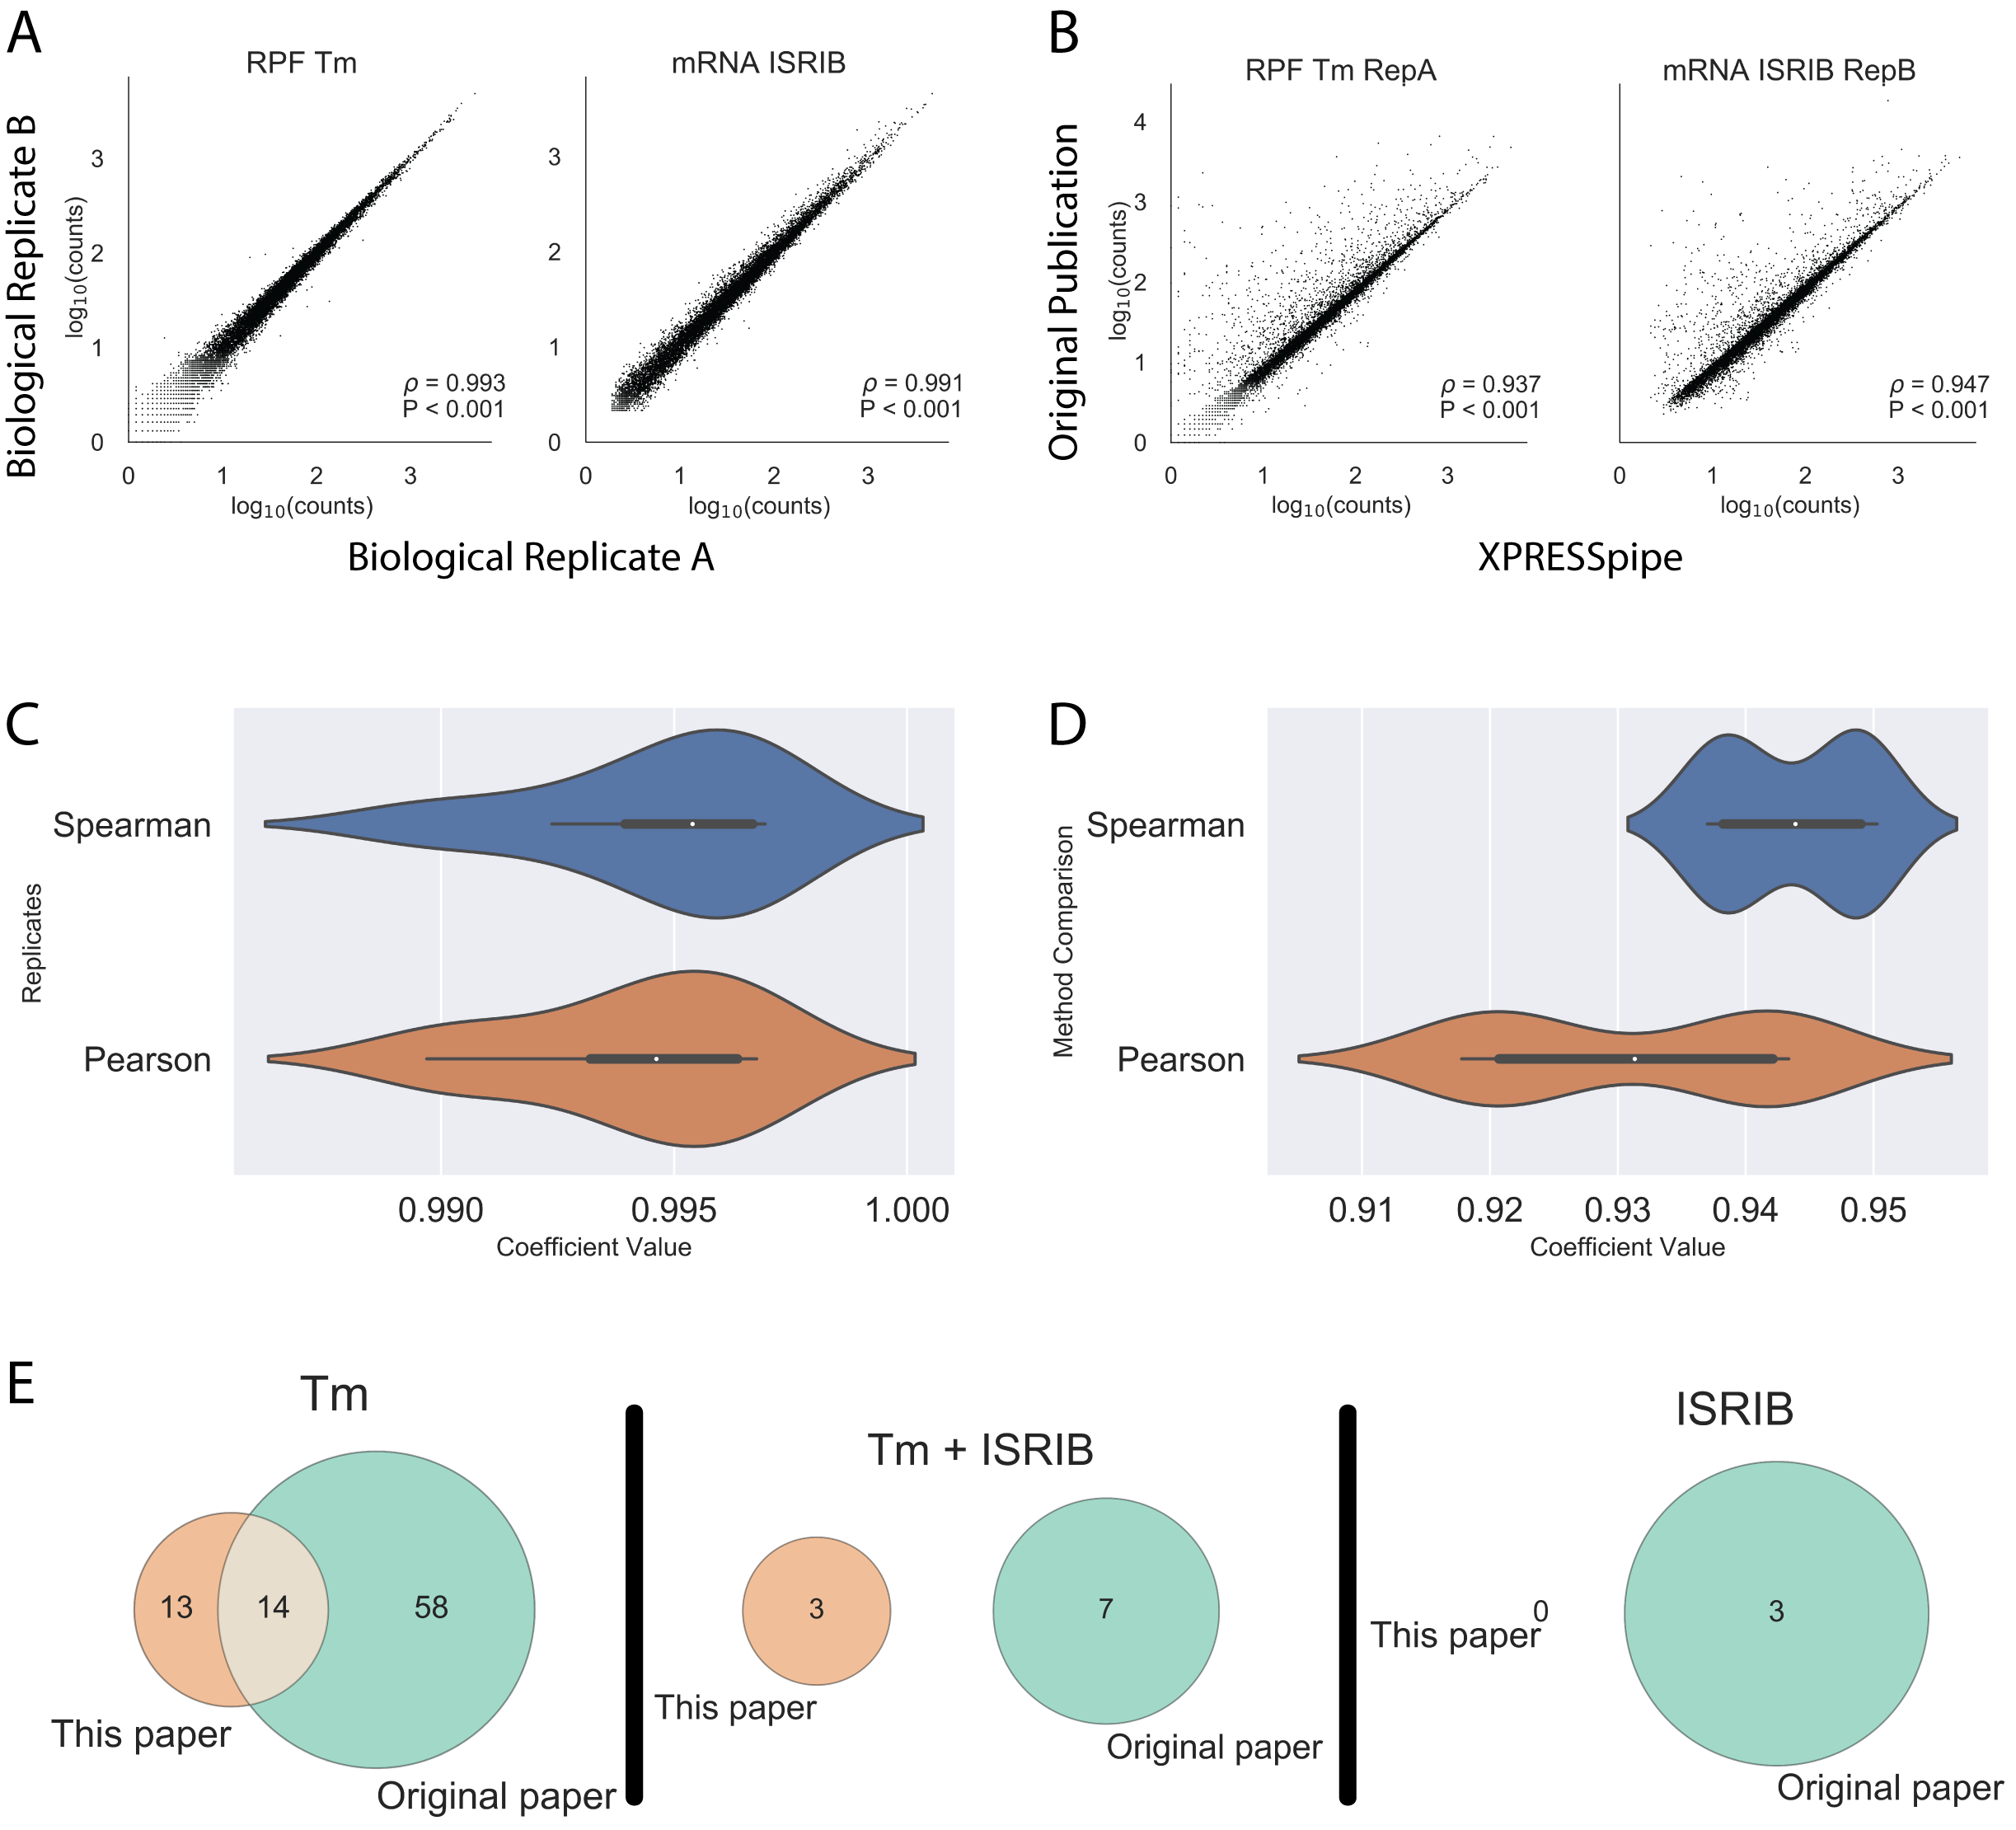
\includegraphics[width=160mm]{figures/xpresspipe_figure2.png}
  \caption{Broad sample quality control and comparision to original processing. A) Cross-processing comparisions between original manuscript and XPRESSpipe. B) Intra-processing comparisions between replicates for XPRESSpipe processing. Note: All R values reported are Spearman R values. All axes are log\textsubscript{10}(counts).}
  \label{fig:figure2}
\end{figure}

Similar canonical targets of translational regulation during ISR were identified in the XPRESSpipe-processed data compared to the original study. These targets include ATF4, ATF5, PPP1R15A, and DDIT3 (Figure \ref{fig:figure3}A-C, highlighted in purple) \cite{isrib_riboseq}. Of note, the fold-change in ribosome occupancy of ATF4 (6.74) from XPRESSpipe-processed samples closely mirrored the estimate from the original publication (6.44). Other targets highlighted in the original study \cite{isrib_riboseq}, such as ATF5, PPP1R15A, and DDIT3 also demonstrated increases in their ribosome occupancy fold-changes as compared to the original processing (XPRESSpipe: 5.82, 2.46, and 3.27; respectively. Original: 7.50, 2.70, and 3.89; respectively) (Figure \ref{fig:figure3}A). Similar to the originally processed data, all of these changes in ribosome occupancy return to about-normal levels during Tm + ISRIB co-treatment (Figure \ref{fig:figure3}B). Additional ISR uORF targets highlighted in the study (highlighted in green in Figure \ref{fig:figure3}A-C) also mirrored changes in translational and transcriptional regulation across the conditions from the original study. \par

In the original study, the genes translationally down-regulated genes were not discussed. However, re-analyzing these data with the updated XPRESSpipe methodology identifies some genes that may play a role in the neurodegenerative effects of ISR and the neuroprotective properties of ISRIB and that were not identified as significantly down-regulated in the original analysis. For example, one would expect putative targets related to neurodegeneration and recovery to be significantly translationally down-regulated during ISR and that these same targets would show recovery towards an untreated state during the ISR + ISRIB treatment. Using this paradigm as a guide, we identified eleven genes following this pattern of translational regulation, as listed in Table \ref{tab:targets} (descriptions sourced from https://www.genecards.org/, https://www.ncbi.nlm.nih.gov/gene/, and https://www.uniprot.org/uniprot/; annotations accessed 27 Jun 2019) (Figure \ref{fig:figure3}D). These targets act as interesting putative targets for further follow-up in a model better mirroring the neurological environment than HEK-293T cells. Further analysis of these potential hits is strengthened by investigating read pile-ups along these genes in IGV \cite{igv} (Figure \ref{fig:supplement3}). This is an important consideration as use of CircLigase in the library preparation can bias certain reads' incorporation in sequencing libraries \cite{circligase_bias}. Distributed footprint coverage is observed across transcripts for all highlighted genes; however, while certain samples appear to be down-regulated in these plots, specific regluation should not be inferred from this information as it has not been sample normalized. However, interestingly, 4 out of the 11 hits passing this strict pattern threshold are strongly annotated as neurological in some manner, and another 2 have mild to moderate neurological annotations. This provides further support to these particular hits for future follow-up for the role in ISR and ISRIB's ability to be neuroprotective by modulating these genes.

For example, SLC1A1 is a glutamine transporter vital for neurotransmission and maintaining glutamine homeostasis. Deficits in this transporter can lead to neurotoxic levels of glutamine within a cell. This transporter is densely expressed throughout the brain \cite{slc1a1_neurotoxic}. Down-regulation of SLC1A1 has already been implicated in diseases such as neurodegenerative diseases caused by mutations in the eukaryotic translation initiation factor 2B subunit epsilon (eIF2B5) \cite{eif2b_neuroprotective}. ISR operates by a similar mechanism, where eIF2$\alpha$ is phosphorylated and a general translation effect is observed \cite{isrib_riboseq, isrib_structure}. This suggests that SLC1A1 abundance control by translation initiation factors is key in an array of neurological conditions and may be partially responsible for the neurodegeneration observed in prolonged ISR conditions. ISRIB's neuroprotective descriptions may therefore stem from a recovery of SLC1A1 levels to wild-type levels which in turn helps regulate glutamine levels. Glutamate transporters, like SLC1A1, have even been implicated in preventing neurotrauma within the first few minutes of insult \cite{slc1a1_neurotoxic}. Within 1 hour of ISR-induction in the focus study \cite{isrib_riboseq}, there was a large decrease in translation efficiency of SLC1A1, suggesting that a rapid disruption or recovery in a vital transporter may play a role in these neurodegenerative and neuroprotective properties.


\begin{figure}
\centering
  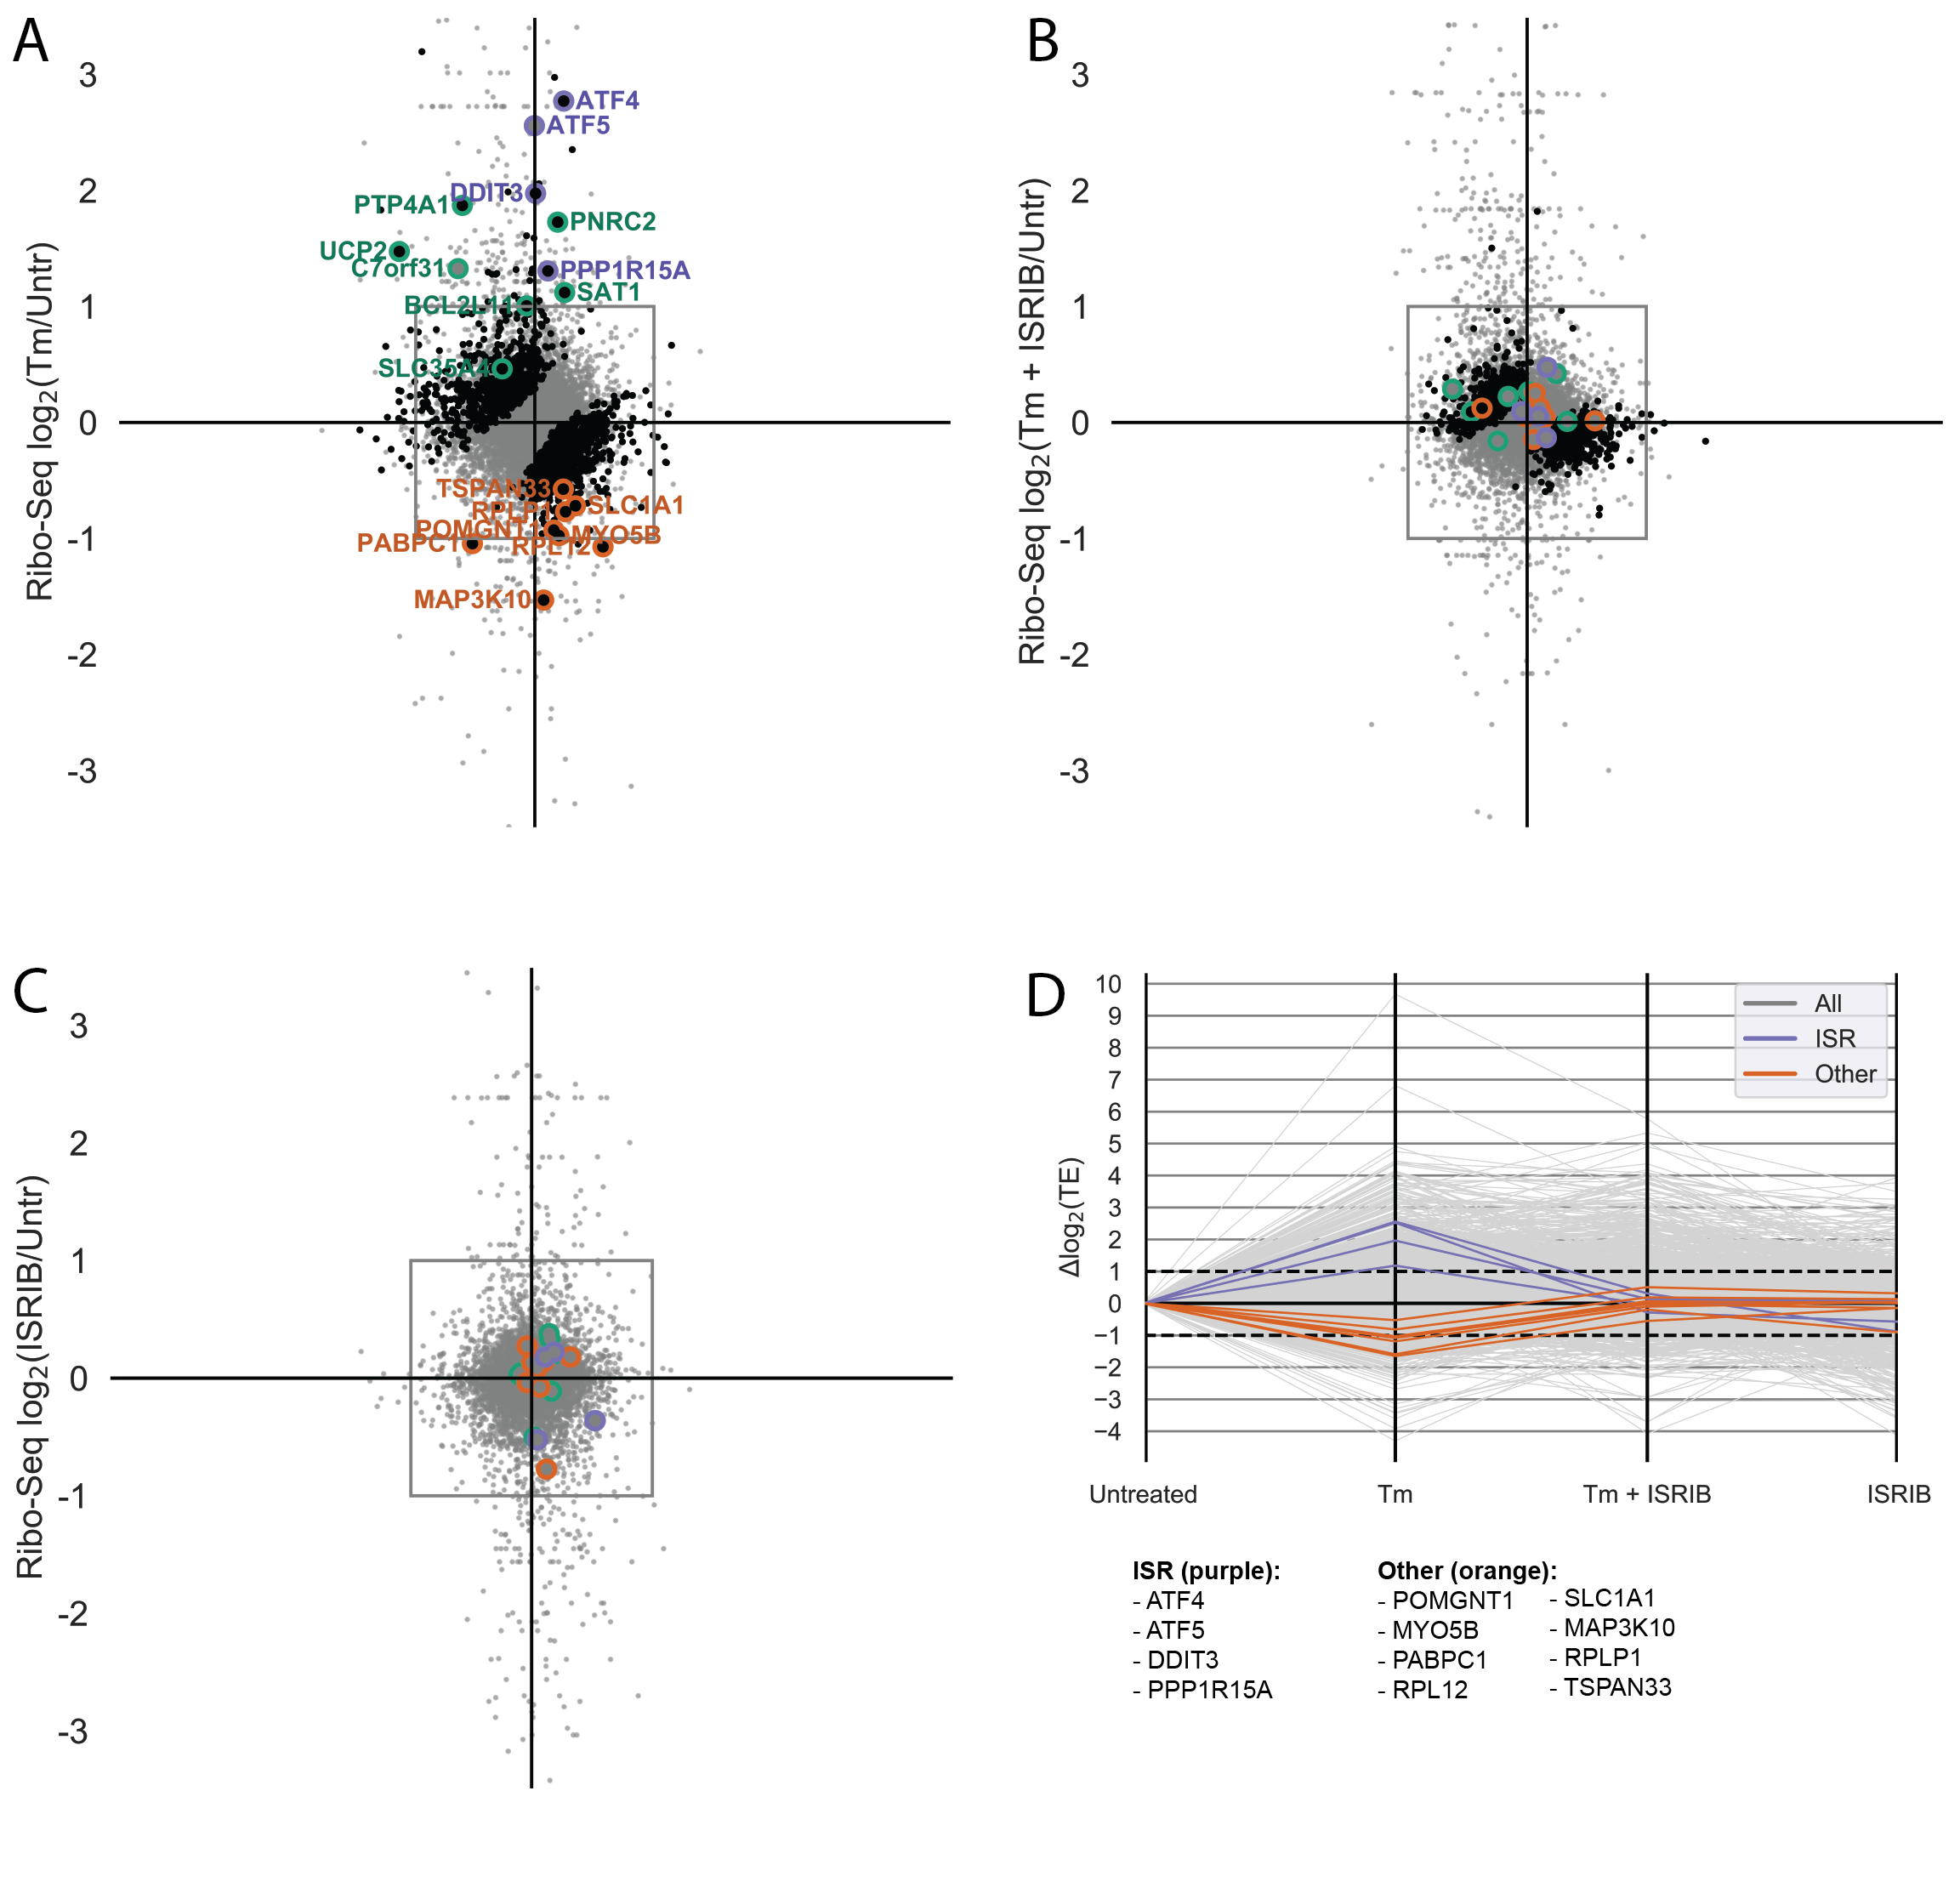
\includegraphics[width=180mm]{figures/xpresspipe_figure3.png}
  \caption{Biological validation and insight into previously published ISR model ribosome profiling data. A-C) Fold change for each drug condition compared to untreated for the ribosome profiling and RNA-seq data. ISR canonical targets highlighted in original study are in purple. Genes with uORFs effected by ISR as highlighted in the original study are highlighted in green. Changes in ribo-seq and mRNA-seq where calculated by DESeq2. Genes with statistically significant changes in translation efficiency for each condition as calculated by DESeq2 are highlighted in black. Points falling outside of plotted range are not included. D) Changes in log\textsubscript{2} Translation Efficiency (TE) compared to Untreated for each drug condition for each of the translationally down-regulated genes passing previous discussed thresholding paradigms. Grey lines are all genes, purple lines indicate ISR canonical targets from original study, orange lines are all genes fitting a strict thresholding paradigm to identify genes that experience a 2-fold or greater increase in TE from Tm treatment to Tm + ISRIB treatment.}
  \label{fig:figure3}
\end{figure}

\captionof{table}{Translationally down-regulated genes during acute Tm treatment and recovered regulation during Tm + ISRIB treatment.}
\begin{tabular}{p{2.5cm}p{15.5cm}}
 \textbf{Gene Name} & \textbf{Relevant Description} \\
 \hline
 POMGNT1 & Participates in O-mannosyl glycosylation. Mutations have been associated with muscle-eye-brain diseases and congenital muscular dystrophies. Expressed especially in astrocytes, as well as in immature and mature neurons. Expressed across brain stem cells. \\
 \hline
 MYO5B & May be involved in plasma membrane recycling. Identified in original ISRIB study. No neurological related annotations. \\
 \hline
 PABPC1 & Promotes ribosome recruitment and translation initation. May contribute to mRNA stability. No neurological related annotations. \\
 \hline
 RPL12 & Ribosomal subunit. No neurological related annotations. \\
 \hline
 ARNTL2 & Helix-loop-helix transcription factor. Expressed throughout the brain, including in the thalamus, hypothalamus, and amygdala. Plays important roles in adaptations to low atmospheric and cellular oxygen levels. \\
 \hline
 SLC1A1 & Dense expression in substantia nigra, red nucleus, hippocampus, and cerebral cortical layers. Member of high-affinity glutamate transporter. In brain, crucial for terminating postsynaptic action of the neurotransmitter glutamate. Responsible for maintaining glutamate concentrations below neurotoxic levels. \\
 \hline
 MAP3K10 & Functions in JNK signaling, reportedly involved in nerve growth factor induces neuronal apoptosis. Expressed in the cerebral cortex. Activates NEUROD1, which promotes neuronal differentation. \\
 \hline
 RPLP1 & Ribosome subunit. Evidence for stem cell and embryonic expression in cerebral cortex. \\
 \hline
 TMEM54 & Unannotated transmembrane protein. \\
 \hline
 AL358472.7 & Unannotated membrane protein. Nonsense mediated decay paralog of JTB, which plays a role in regulation of cell proliferation. \\
 \hline
 TSPAN33 & Plays a role in normal erythropoiesis and regulates maturation and trafficking of ADAM10, a metalloprotease. Negatively regulates Notch activity by way of its regulation of ADAM10. Notch signaling is vital to neurogenesis. \\
 \label{tab:targets}
\end{tabular}
\newline


\subsubsection{Performance Validation Using TCGA Data}
To validate the general design and reliability of the XPRESSpipe pipeline, we processed raw TCGA sequence data using XPRESSpipe and compared the output count values to those publicly available through TCGA. Spearman R values for the selected samples ranged from 0.95 - 0.96 (Figure \ref{fig:figure4}), indicating general integrity of pipeline design according to TCGA standards. The differences in reported counts can be accounts by a couple key differences. For example, the presented XPRESSpipe-processed files used the Homo sapiens GRChv96 reference transriptome, while the original count data used GRChv79 reference transriptome. As seen from Figure \ref{fig:supplement4}A, the use of a different transcriptome reference can cause vast variation alone between final quantified data. For example, the GDC pipeline cites Ensembl build GRCh38 version 79, while the most recent version of this reference is version 96. In the 4 years difference between these versions, significant advances have been made in our understanding of transcribed regions of the genome. Between versions 95 and 96 alone (version 95 published 24 Nov 2018, version 96 published 13 Mar 2019), approximately 32,259 additional records (quantified by difference in line numbers between the files) were added or changed. The plot enclosed in maroon was processed with XPRESSpipe setting set to the same as presented in the TCGA published pipeline. The plot enclosed in green used XPRESSpipe default settings. Another source of variation arises from the use of Ensembl canonical transcripts only during quantification. TCGA-processed data used an unmodified transcriptome reference file, therefore, use of this modified GTF will add variation as quantifications are constained to a single transcript version of a given gene. Interestingly, even using XPRESSpipe settings closest to the TCGA pipeline and using the same genome and transcriptome version resulted in some variation (Figure \ref{fig:supplement4}A, plot enclosed in maroon). By performing a closer analysis of these differences, we see that virtually all genes exhibiting differences between the processing methods are pseudogenes (Figure \ref{fig:supplement4}B), with the TCGA pipeline quantifying more pseudogenes. While pseudogene expression is real and often biologically relevant, high levels, particularly 10-fold differences, of pseudogene expression are less likely, indicating a slightly more reliable quantification by way of XPRESSpipe.


\begin{figure}
\centering
  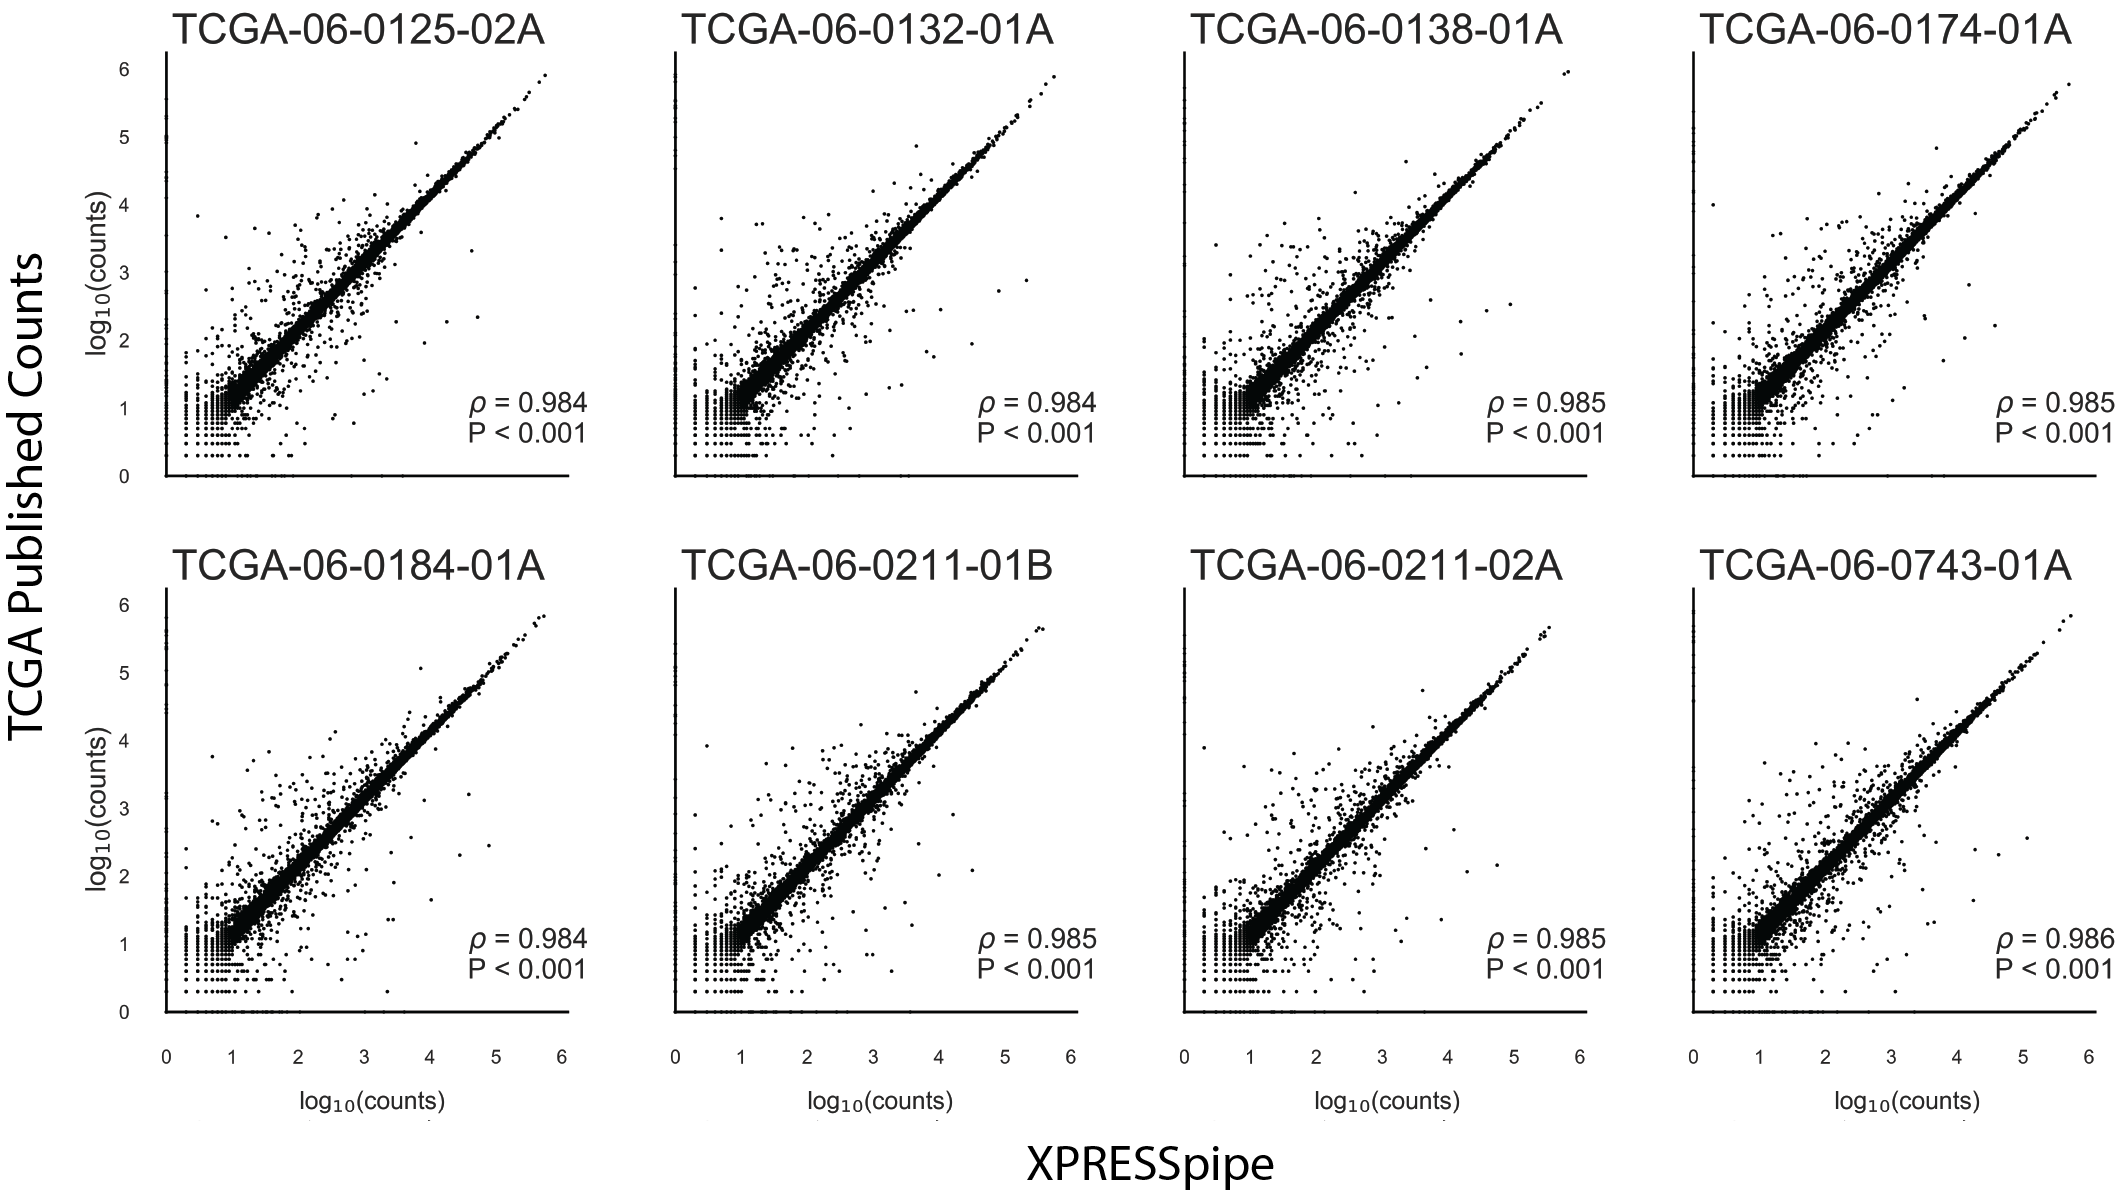
\includegraphics[width=180mm]{figures/xpresspipe_figure4.png}
  \caption{Pipeline validation using publicly available TCGA count data. Correlations were calculated between publicly available count data from TCGA samples and the XPRESSpipe on the sequence count data. Note: All R values reported are Spearman R values. All axes are log\textsubscript{10}(counts).}
  \label{fig:figure4}
\end{figure}


\subsubsection{Cost Analysis}
XPRESSpipe functions can be computationally intensive and thus super-computing resources are recommended. Many universities provide super-computing resources to their staff and students; however, in cases where these resources are not available, servers such as Amazon Web Services (AWS) (https://aws.amazon.com/) can be used to process sequencing data using XPRESSpipe. For example, the ribosome profiling dataset of 32 raw sequence files used in the study was processed using the University of Utah's Center for High Performance Computing resources. Run statistics can be found in Table \ref{tab:chpc_performance}.

% UPDATE BEFORE SUBMISSION ONCE QUALITY CONTROL STABLE AND CHECK CONVERSIONS\
UPDATE
\captionof{table}{XPRESSpipe processing statistics for dataset GSE65778.}
\begin{tabular}{p{5cm}p{3cm}}
\textbf{Metric} & \textbf{Value} \\
\hline
 Elapsed Real Time & 09h32m58s \\
 \hline
 Total CPU Time & 1d10h11m42s  \\
 \hline
 Allocated CPUs & 16 \\
 \hline
 Allocated Memory per Node & 62.50GB \\
 \hline
 Maximum RAM of all tasks & 62.60GB \\
 \label{tab:chpc_performance}
\end{tabular}
\newline

Based on these metrics, if HPC services weren't locally available for a user, one could use Amazon Web Services to process the data for relatively little money. For a comparable run, storage cost would amount to around 14 USD/month on Amazon S3 storage and compute cost for a similar computational node for the given elapsed time would cost around 7.50 USD using Amazon EC2 On-Demand m5.4xlarge node (however, significantly reduced rates are available if using Spot instances or by using the free tier; calculations were performed 28 Jun 2019).


\section{Discussion}
We have described herein a new software suite, XPRESSyourself, a collection of tools to aid in expression data processing and analysis. While RNA-seq technologies are becoming more and more mature, standardized protocols are lacking. This is problematic when individuals or groups may not be using the most up-to-date methods or be aware of particular biases or measures of quality control required to produce a reliable, high-quality sequencing study. XPRESSpipe handles these issues through continuous curation by XPRESSyourself team members to ensure the pipeline is utilizing the best-performing software tools in sequencing as measured by peer-reviewed benchmarking studies. It also outputs all necessary quality control metrics so that the user can quickly assess quality and identify any systematic problems or technical biases that may be present in their samples. \par

An additional problem XPRESSpipe addresses is the incorrect use of these software tools, which is especially important  for those coming from a non-computational background. XPRESSyourself will dissolve this barrier to entry for most users so that they can process and analyze their data immediately upon receipt of the raw data and only requires simple programming knowledge covered by a variety of free online programs (such as https://www.codecademy.com/learn/learn-the-command-line). These users can also be assured they are using the most up-to-date standard for RNA-seq processing and analysis. \par

Tools previously missing from the general ribosome profiling toolkit have also been added within XPRESSyourself. This includes GTF truncation of transcripts in a recursive manner over CDS space and rRNA probe design aids for removing contaminating rRNA sequences in ribosome profiling libraries that are difficult to remove with commercial kits. \par

We demonstrated the utility of the XPRESSyourself toolkit by re-analyzing a publicly available ribosome profiling dataset. From this analysis, we identified putative hits that may contribute to the neurodegenerative effects of integrated stress response (ISR) and how the molecule ISRIB may be acting on these hits to act as a neuroprotective agent. This additionally highlights the importance of re-analyzing older datasets with more current methods, as over time methodologies improve to reduce errors. We also showed the capability of quickly processing data on TCGA data. These principles are transferable to new datasets and XPRESSyourself will have individuals and labs take sequence processing and analysis into their own hands rapidly process and analyze their data, save money, and put missing or incomplete computational tools required for ribosome profiling and RNA-seq into the hands of the average user. Additionally, usage of XPRESSyourself containers will aid in reproducibility in science and make transparent methods easy to incorporate into associated publications. \par

While admittedly the XPRESSyourself pipeline may be somewhat more time and computationally intensive than other pipelines, the trade-off is higher quality alignments and quantification, and unless analyzing thousands of samples, is generally not too expensive or time-consuming.


\section{Conclusions}
With the adoption of this pipeline, the field of high-throughput sequencing, particularly within ribosome profiling, can continue to standardize the processing protocol for sequencing data and eliminate some of the variability that comes from using a variety of software packages for various steps during read processing. XPRESSpipe will act as a flexible pipeline that will be updated with the best performing packages as future tools are created and benchmarks performed. Additionally, various tools missing from the ribosome profiling and RNA-seq communities have been added as part of this pipeline. With these tools, such as the GTF modification sub-module, genome reference formatting and curation is automated and accessible to the public. Further, by using this pipeline on publicly available data, we highlight XPRESSpipe's utility in being able to re-process publicly available data or personal data to uncover novel biological patterns quickly. Adoption of this tool will aid the average scientist is quickly accessing their data, using the highest-quality methods.


\section{Materials and Methods}

\subsection{Software Dependencies}
A list of dependencies required for XPRESSpipe is listed in Table \ref{Tab:software_pipe}. Dependencies for XPRESSplot are listed in Table \ref{Tab:software_plot}.

% Software dependencies table
\captionof{table}{Summary of dependency software, accession location, and purpose in the XPRESSpipe package.}
\begin{tabular}{p{2.4cm}p{7.5cm}p{3cm}}
 \textbf{Package} & \textbf{Purpose} & \textbf{Reference} \\
 \hline
 Python & Primary language & \\
 \hline
 R & Language used for some statistical modules & \\
 \hline
 fastp & Read pre-processing & \cite{fastp} \\
 \hline
 STAR & Reference curation and read alignment & \cite{star} \\
 \hline
 samtools & Alignment file manipulation & \cite{samtools} \\
 \hline
 bedtools & Alignment file manipulation & \cite{bedtools} \\
 \hline
 Cufflinks & Read quantification (primary) & \cite{cufflinks} \\
 \hline
 HTSeq & Read quantification & \cite{htseq} \\
 \hline
 FastQC & Quality Control & \cite{fastqc} \\
 \hline
 MultiQC & Quality Control & \cite{multiqc} \\
 \hline
 pandas & Data manipulation & \cite{pandas} \\
 \hline
 numpy & Data manipulation & \cite{numpy1, numpy2} \\
 \hline
 scipy & Data manipulation & \cite{scipy} \\
 \hline
 sklearn & Data manipulation & \cite{sklearn} \\
 \hline
 matplotlib & Plotting & \cite{matplotlib} \\
 \hline
 XPRESSplot & Normalization and matrix manipulation & This paper \\
 \hline
 dupRadar & Perform library complexity calculations & \cite{dupradar} \\
 \hline
 DESeq2 & Perform differential expression analysis & \cite{deseq2} \\
 \label{Tab:software_pipe}
\end{tabular}
\newline

% Software dependencies table
\captionof{table}{Summary of dependency software, accession location, and purpose in the XPRESSplot package.}
\begin{tabular}{p{2.4cm}p{7.5cm}p{3cm}}
 \textbf{Package} & \textbf{Purpose} & \textbf{Reference} \\
 \hline
 Python & Primary language & \\
 \hline
 R & Language used for some statistical modules & \\
 \hline
 pandas & Data manipulation & \cite{pandas} \\
 \hline
 numpy & Data manipulation & \cite{numpy1, numpy2} \\
 \hline
 scipy & Data manipulation & \cite{scipy} \\
 \hline
 matplotlib & Plotting & \cite{matplotlib} \\
 \hline
 seaborn & Plotting & \cite{seaborn} \\
 \hline
 plotly & Plotting & \cite{plotly} \\
 \hline
 sklearn & Data manipulation & \cite{sklearn} \\
 \hline
 GEOparse & Access GEO data & \cite{geoparse} \\
 \hline
 DESeq2 & Perform differential expression analysis & \cite{deseq2} \\
 \hline
 sva & Perform batch correction for known effects with the ComBat function & \cite{sva} \\
 \label{Tab:software_plot}
 \end{tabular}
 \newline

\subsection{GTF Modification}
Protein coding genes are identified by the ``protein\_coding" annotation within \texttt{attribute} column of the GTF file.
UPDATE
Longest transcripts are determined by calculating the exon space for each transcript associated with a given \texttt{gene\_id}. If a pre-mature stop is annotated within a transcript, that is considered the end-point of the transcript length. \par
Truncation is performed by identifying the 5' and 3' end of each transcript and modifying the given coordinates to reflect the given truncation amounts. The amounts to be truncated can be modulated by the user; however, suggested ranges are 45 nt from the 5' end and 15 nt from the 3' end, set as the default parameters for the function \cite{ingolia_meth}. As a given CDS may be less than the specified amounts, the function will recursively search CDS by CDS until the full truncated amount is trimmed.

\subsection{Normalization}
Equations 1-4 reflect the design of the normalization functions within XPRESSplot.

  \begin{equation}
    RPM = \frac{(\#\ number\ reads\ per\ gene)\ \cdot\ 1e6}{(\#\ mapped\ reads\ per\ sample)}
  \end{equation}
  \begin{equation}
    RPKM = \frac{(\#\ number\ reads\ per\ gene)\ \cdot\ 1e6\ \cdot\ 1e3}{((\#\ mapped\ reads\ per\ sample)\ \cdot\ (gene\ length\ (bp))}
  \end{equation}
  \begin{equation}
    FPKM = \frac{(\#\ number\ fragments\ per\ gene)\ \cdot\ 1e6\ \cdot\ 1e3}{(\#\ mapped\ fragments\ per\ sample)\ \cdot\ (gene\ length\ (bp))}
  \end{equation}
  \begin{equation}
    TPM = \frac{(\#\ number\ fragments\ per\ gene)\ \cdot\ 1e3\ \cdot\ 1e6}{(gene\ length\ (bp))\ \cdot\ (\#\ mapped\ fragments\ per\ sample)}
  \end{equation}

\subsection{Quality Control Summary Plotting}
Summary plots are created using pandas \cite{pandas} and matplotlib \cite{matplotlib}. Kernel density plots for library complexity analyses are created using numpy \cite{numpy1, numpy2} and scipy's \texttt{gaussian\_kde} function \cite{scipy}.

\subsection{Metagene Estimation}
Metagene calculations are performed by determining the meta-genomic coordinate \textit{M} for each aligned read, where \textit{L\textsubscript{e}} is the leftmost coordinate of the mapped read and \textit{r} is the length of the mapped read. \textit{S} denotes the start coordinate for the transcript and \textit{l\textsubscript{e}} is the cumulative length of all exons for the given transcript. The subscripted \textit{e} indicates the coordinate is relative to exon space, where intron space is not counting in the coordinate relative to the start of the transcript. Required inputs are an indexed BAM file and an unmodified GTF reference file. For each mapped coordinate, the metagene position is calculated as:
\begin{equation}
\textit{M} = \frac{|(L\textsubscript{e}\ +\ \frac{1}{2}r)\ -\ S|\ \cdot\ 100}{\textit{l\textsubscript{e}}}
\end{equation}

In the case where a mapped coordinate falls within multiple genes, a penalty is assigned as:
\begin{equation}
  \textit{c} = \frac{1}{\textit{n}}
\end{equation}
Where \textit{c} is the count score for a given meta-position and \textit{n} is the number of different transcripts a given coordinate mapped. To be counted or factored into the penalty, the meta-position coordinate must fall within exon space.

\subsection{Periodicity}
\textit{p} is the distance from the start coordinate, \textit{L\textsubscript{e}} is the leftmost coordinate of the mapped read, \textit{r} is the length of the mapped read, and \textit{S} denotes the start coordinate for the transcript. The superscript signs associated with \textit{p} indicate strandedness and the subscript \textit{e} indicates the coordinate is relative to exon space. Only reads 28-30 nucleotides long are considered in this analysis. The penalty is calculated in the same manner as in the \texttt{metagene} sub-module.
\begin{equation}
  \textit{p}\textsuperscript{+} = (\textit{L}\textsubscript{e}\ +\ \textit{r} - 16)\ -\ \textit{S}
\end{equation}
\begin{equation}
  \textit{p}\textsuperscript{-} = \textit{S}\ -\ (\textit{L}\textsubscript{e}\ +\ 16)
\end{equation}

\subsection{rRNA Probe}
\texttt{rrnaProbe} works on a directory containing fastqc \cite{fastqc} zip compressed files to detect over-represented sequences for each sample. These sequences are then collated to create consensus fragments. One caveat is that FASTQC collates on exact matching sequences, but these sequences may be 1 nt steps from each other and a single rRNA probe could be used to effectively pull out all these sequences. In order to handle this situation, XPRESSpipe will combine these near matches. A rank ordered list of over-represented fragments within the appropriate length range to target for depletion is then output. A BLAST \cite{blast} search on consensus sequences intended for probe useage can then be performed to verify the fragment maps to an rRNA sequence and is thus a suitable depletion probe.

\subsection{Confidence Interval Plotting}
Confidence intervals within PCA scatterplots generated by XRESSplot are calculated as follows:

\begin{enumerate}
  \item Compute the covariance of the two principle component arrays, \textit{x} and \textit{y} using the numpy.cov() function.

  \item Compute the eigenvalues and normalized eigenvectors of the covariance matrix using the numpy.linalg.eig() function.

  \item Compute the $\theta$ of the normalized eigenvectors using the numpy.arctan2() function and converting the output from radians to degrees using numpy.deg().

  \item Compute the $\lambda$ of the eigenvalues by taking the square root of the eigenvalues.

  \item Plot the confidence intervals over the scatter plot: The center point of the confidence interval is determined from the means of the \textit{x} and \textit{y} arrays. The angle is set equal to $\theta$. The width of the condfidence interval is calculated by
  \[
  \textit{w} = \lambda _{\textit{\scriptsize{x}}}\ \cdot\ \textit{ci}\ \cdot\ 2
  \]
  where \textit{ci} is equal to the corresponding confidence level (i.e. 68\% = 1, 95\% = 2, 99\% = 3). The heighth is similarly computed by
  \[
  \textit{h} = \lambda _{\textit{\scriptsize{y}}}\ \cdot\ \textit{ci}\ \cdot\ 2
  \]
\end{enumerate}

\subsection{Ribosome Profiling Example Data Analysis}
The following xpresspipe command was run to process the raw data, available from GEO. Reference files were taken from Ensembl Human build GRCh38v96.

\begin{lstlisting}[language=bash, caption=Ribosome profiling processing command.]
# Generate reference files
$ xpresspipe curateReference -o $SCRDIR/references/human_reference -f $SCRDIR/references/human_reference -g $SCRDIR/references/human_reference/transcripts.gtf --sjdbOverhang 49 -l -p -t
# Execute pipeline
$ xpresspipe riboseq -i $SCRDIR/input -o $SCRDIR/output -r $REF --gtf $REF/transcripts_LCT.gtf -e isrib_riboprof -a CTGTAGGCACCATCAAT --method RPKM --sjdbOverhang 49
\end{lstlisting}

Only gene names in common between the original data file and XPRESSpipe output were used for the method comparisons. Genes included in all studies were required to have at least 25 counts across samples to be included in the analysis. Correlations and p-values were calculated using the \texttt{scipy.stats.spearman()} function \cite{spearman_rnaseq}. Sample count distributions were plotted using Seaborn where density is indicated by width of plot and boxplot designating interquartile range are plotted \cite{seaborn}. Fold change and translation efficiency plots were created using matplotlib \cite{matplotlib} and pandas \cite{pandas}. Replicates were combined to calculate fold change values and significance between library groups (condition and library type) was calculated using a Benjamini-Hochberg FDR method from \texttt{statsmodels.stats.multitest()} \cite{statsmodels}. Gene coverage profiles were generating using IGV \cite{igv}. Figures and analyses can be reproduced using the associated scripts found at https://github.com/XPRESSyourself/manuscript (DOI: XXXXXX). \par

Translation efficiency was calculated as follows:

\begin{equation}
  \Delta TE = \frac{RPF\textsubscript{\textit{treatment}}}{mRNA\textsubscript{\textit{treatment}}} - \frac{RPF\textsubscript{\textit{untreated}}}{mRNA\textsubscript{\textit{untreated}}}
\end{equation}

\subsection{Cost Analysis}
Cost analysis was performed by accessing run logs from the HPC and using published AWS prices (https://aws.amazon.com/ec2/pricing/on-demand/, https://aws.amazon.com/s3/pricing/, accessed 28 May 2019) to calculate relative cost for a similar run.

\section*{List of abbreviations}
UMI - unique molecular identifier, nt - nucleotide,

\section*{Ethics approval and consent to participate}
Protected TCGA data were obtained through dbGaP project number 21674 and utilized according to the associated policies and guidelines.

\section*{Consent for publication}
Protected TCGA data were obtained through dbGaP project number 21674 and utilized according to the associated policies and guidelines.

\section*{Availability of data and materials}
The source code for these packages will be perpetually open source and protected under the GPL-3.0 license. The code can be publicly accessed and installed from https://github.com/XPRESSyourself. Updates to the software are version controlled and maintained on GitHub. Jupyter notebooks and video walkthroughs are included on https://github.com/XPRESSyourself for guiding a user through use of the packages. Documentation is hosted on readthedocs \cite{readthedocs} at https://xpresspipe.readthedocs.io/en/latest/ and https://xpressplot.readthedocs.io/en/latest/. The publicly available ribosome profiling data are accessible through GEO series accession number GSE65778. TCGA data are accessible through dbGaP accession number phs000178. Code used to create manuscript figures and analyses can be found at https://github.com/XPRESSyourself/manuscript (DOI: XXXXXX).

\section*{Competing interests}
The authors declare that they have no competing interests.

\section*{Funding}
J.A.B. received support from the National Institute of Diabetes and Digestive and Kidney Diseases (NIDDK) Inter-disciplinary Training Grant T32 Program in Computational Approaches to Diabetes and Metabolism Research, 1T32DK11096601 to Wendy W. Chapman and Simon J. Fisher.

\section*{Contributions}
J.A.B. conceptualized and administered the project; performed all investigation, analysis, visualization, and data curation; provisioned computing resources; acquired funding; amd write the original draft for this study. J.A.B. wrote the software and J.R.B. designed and wrote the rRNA Probe sub-module. J.A.B., J.T.M., A.J.B., and Y.O. performed software and documentation validation. J.A.B., J.R.B., M.T.H., and J.G. and developed the methodology. J.P.R, M.T.H., J.G., and A.R.Q. supervised the study. All authors were involved in reviewing and editing the manuscript.

\section*{Acknowledgments}
The authors wish to thank Michael Howard for helpful discussions concerning ribosome profiling and sequencing analysis. The authors also wish to thank Mark Wadsworth, Ryan Miller, and Michael Cormier for helpful discussions on pipeline design. They also wish to thank Cameron Waller for helpful discussions related to pipeline design and analysis. The support and resources from the Center for High Performance Computing at the University of Utah are gratefully acknowledged. The computational resources used were partially funded by the NIH Shared Instrumentation Grant 1S10OD021644-01A1. The results published here are in whole or part based upon data generated by the TCGA Research Network: https://www.cancer.gov/tcga.


\bibliography{manubib}
\bibliographystyle{Science}

\beginsupplement

\begin{figure}
\centering
  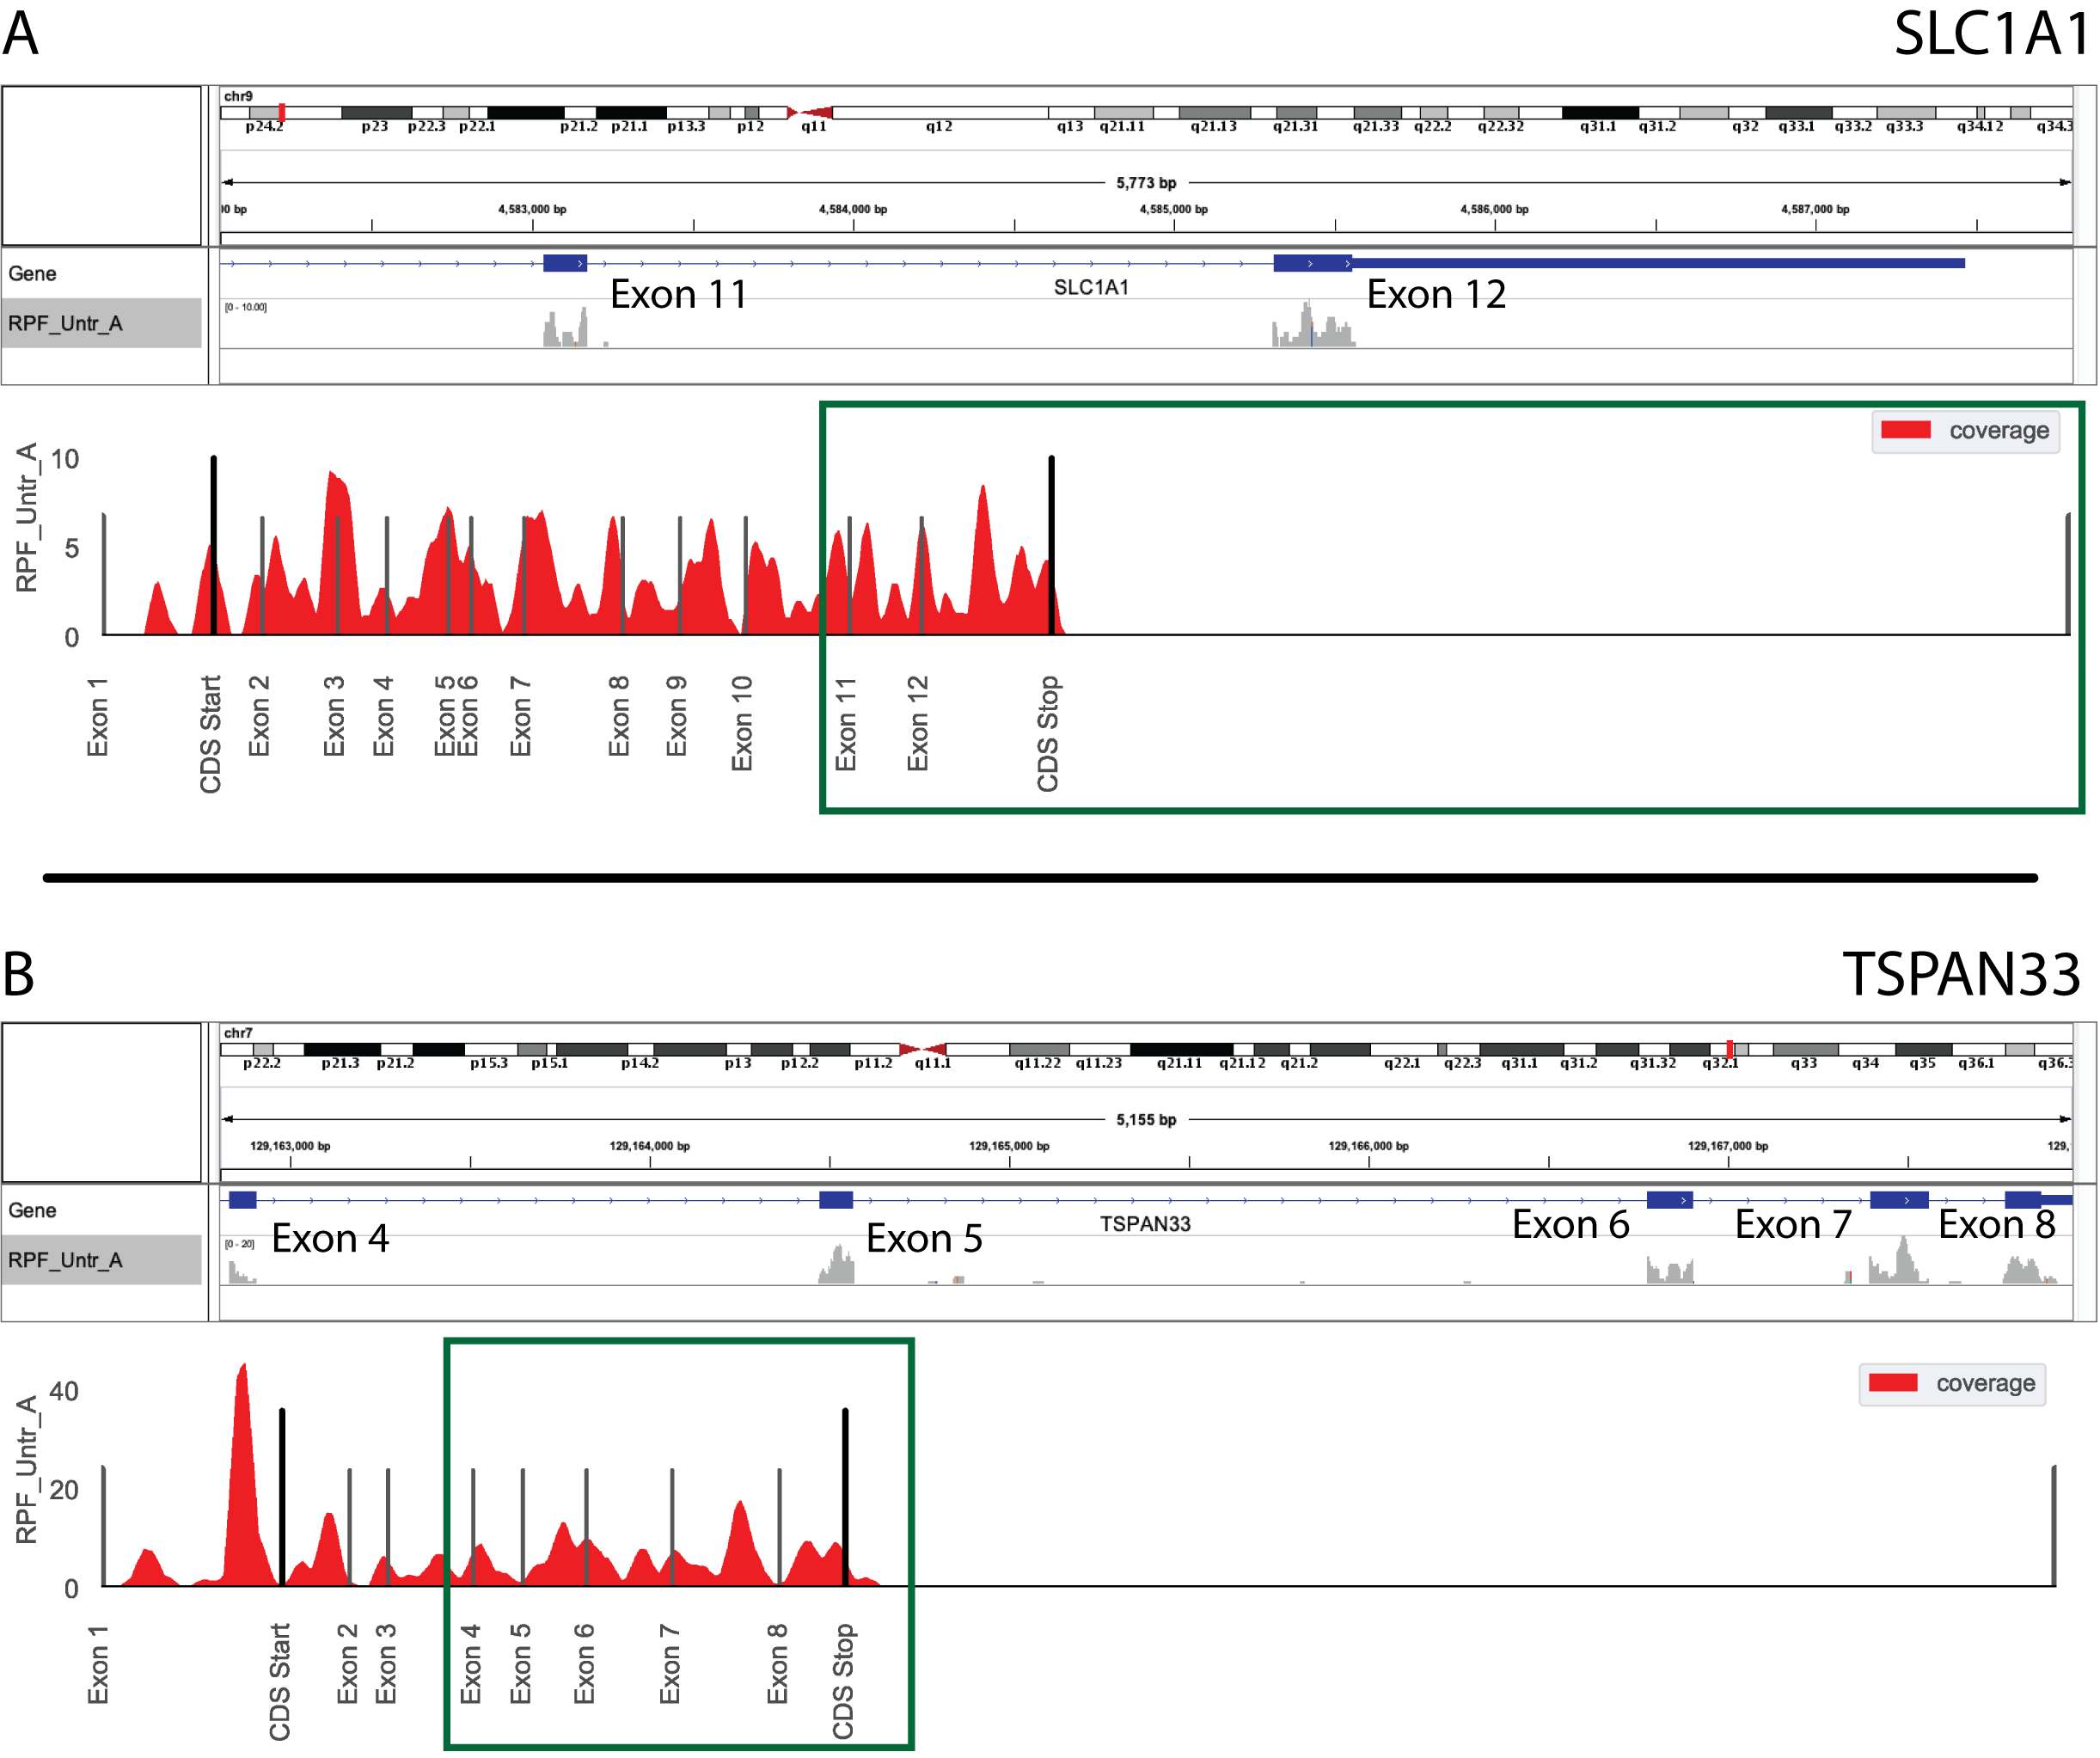
\includegraphics[width=160mm]{figures/xpresspipe_supplement2.png}
  \caption{A sampling of the original counts data plotted against XPRESSpipe-processed data. Selected highlighted genes show consistent differences between processing methods.}
  \label{fig:supplement2}
\end{figure}

\begin{figure}
\centering
  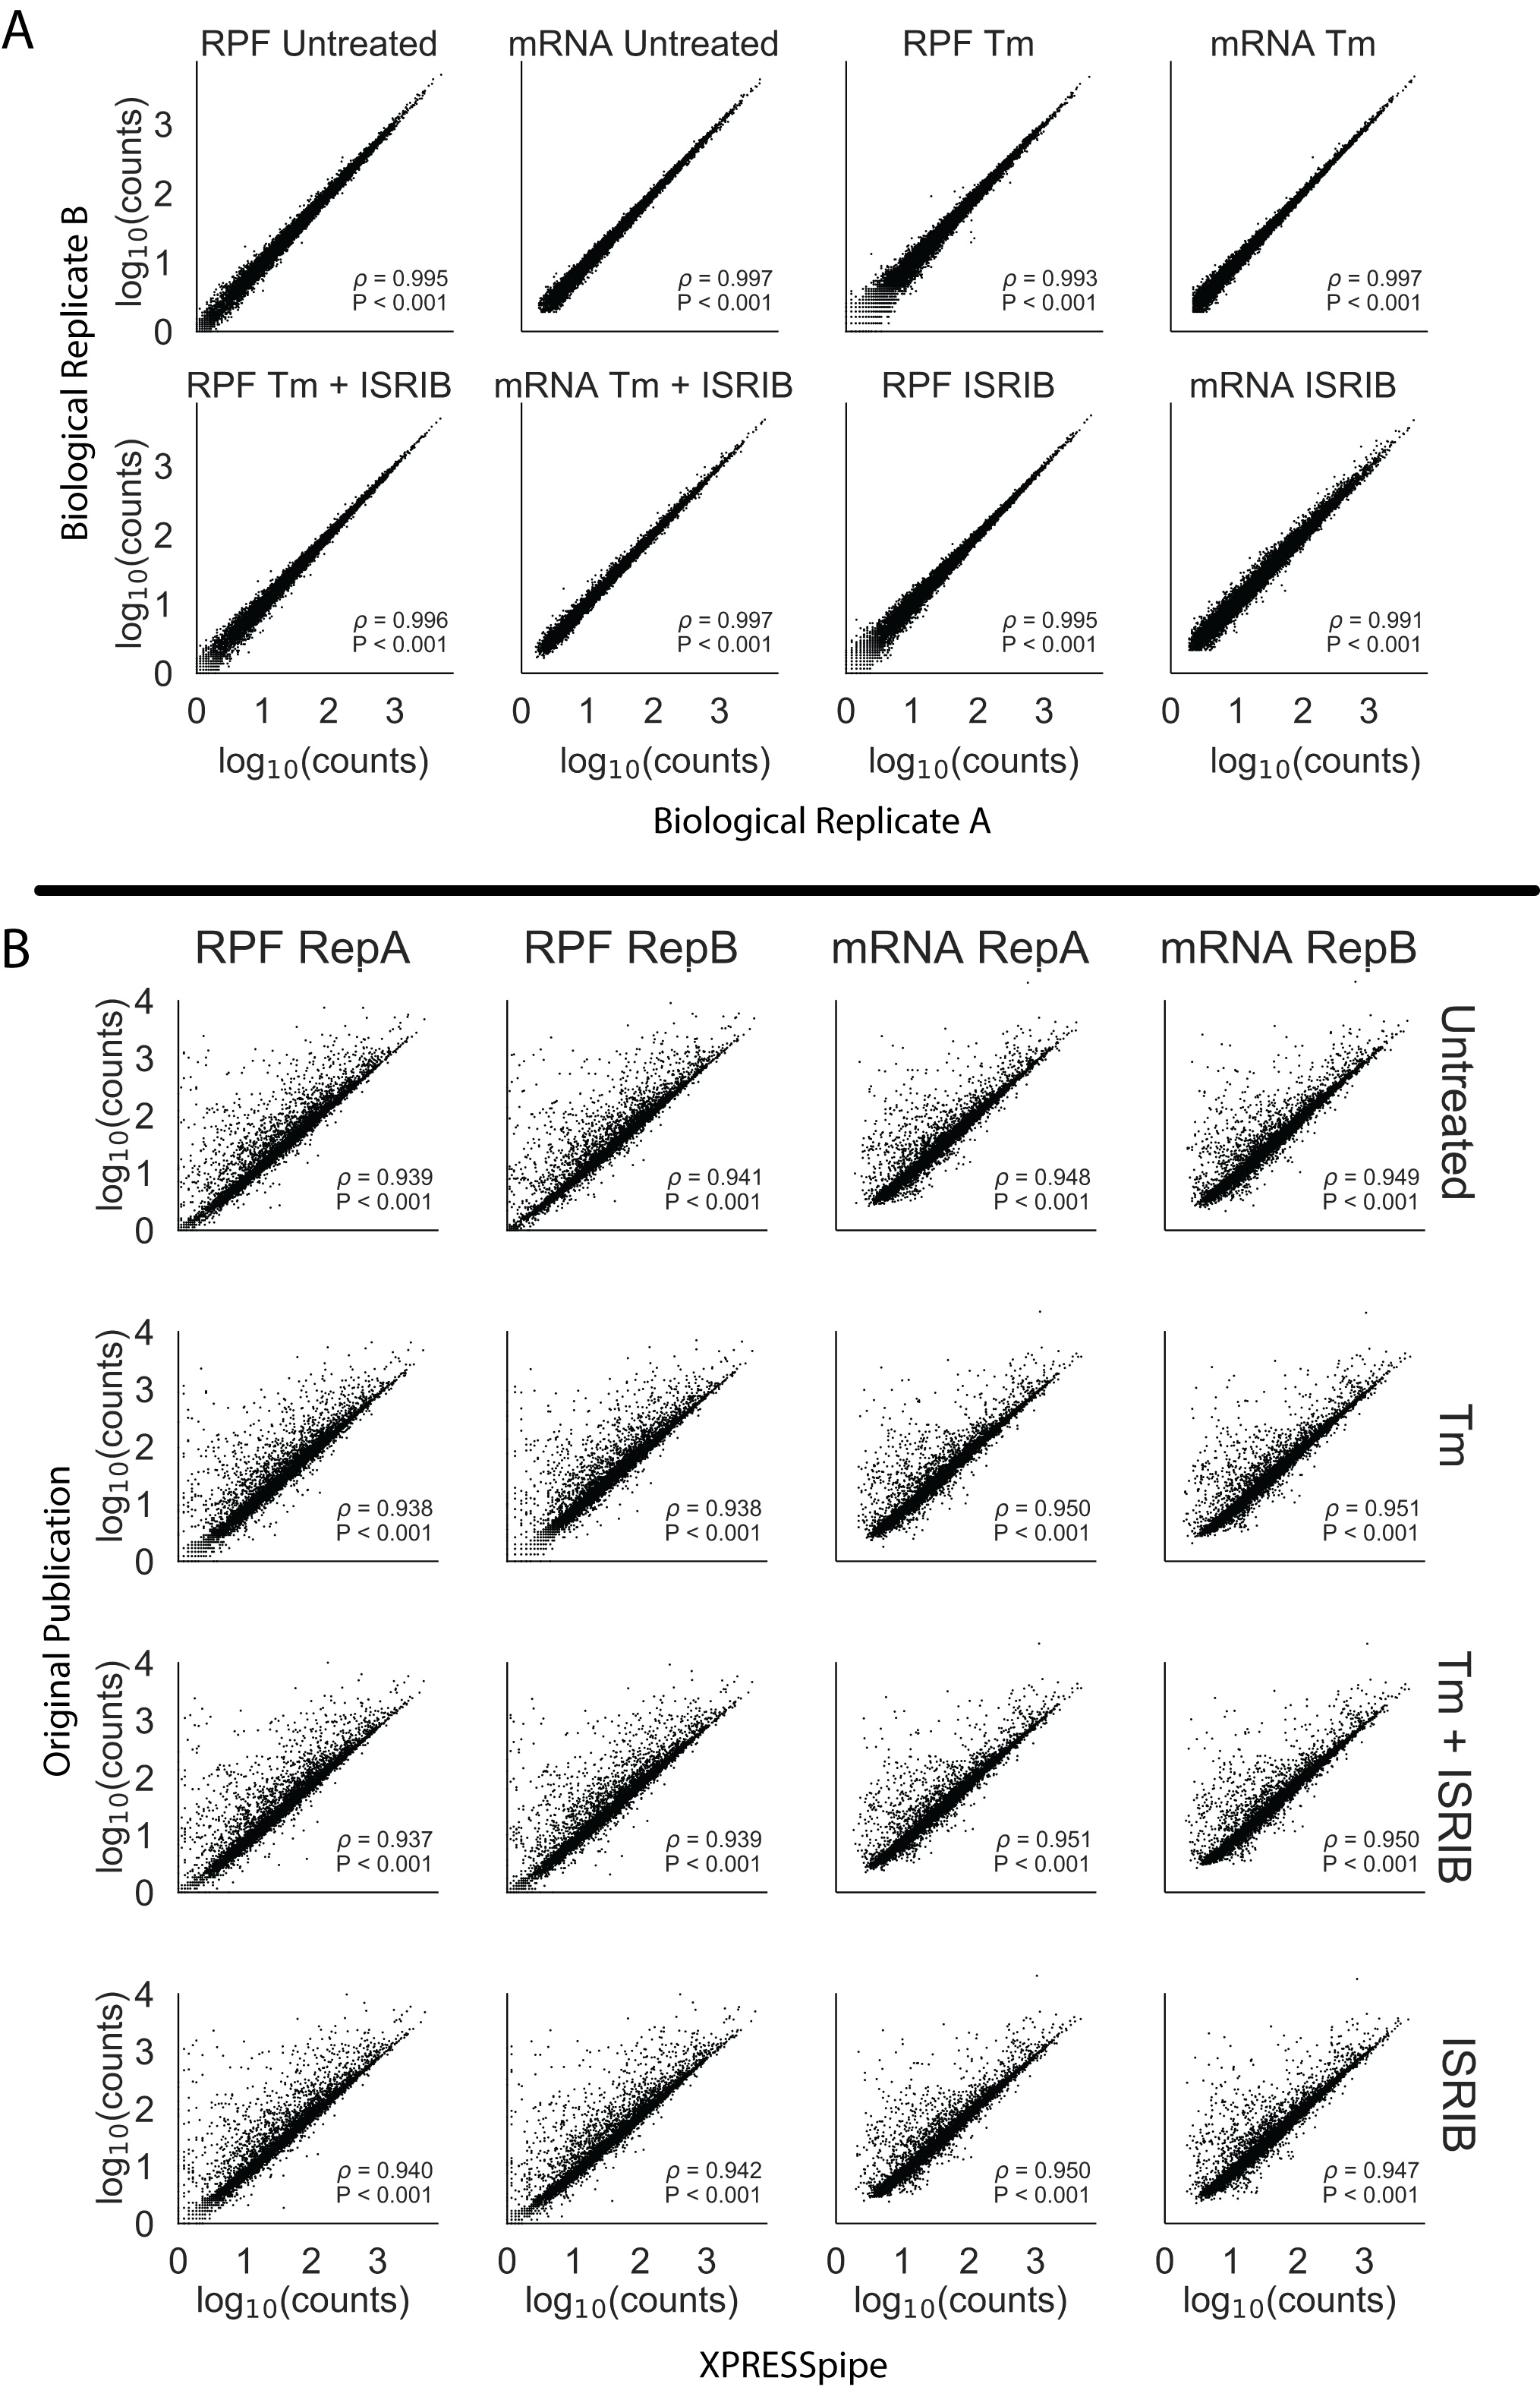
\includegraphics[width=180mm]{figures/xpresspipe_supplement3.png}
  \caption{IGV coverage plots for strongest neurologically annotated genes passing strict thresholding.}
  \label{fig:supplement3}
\end{figure}

\begin{figure}
\centering
  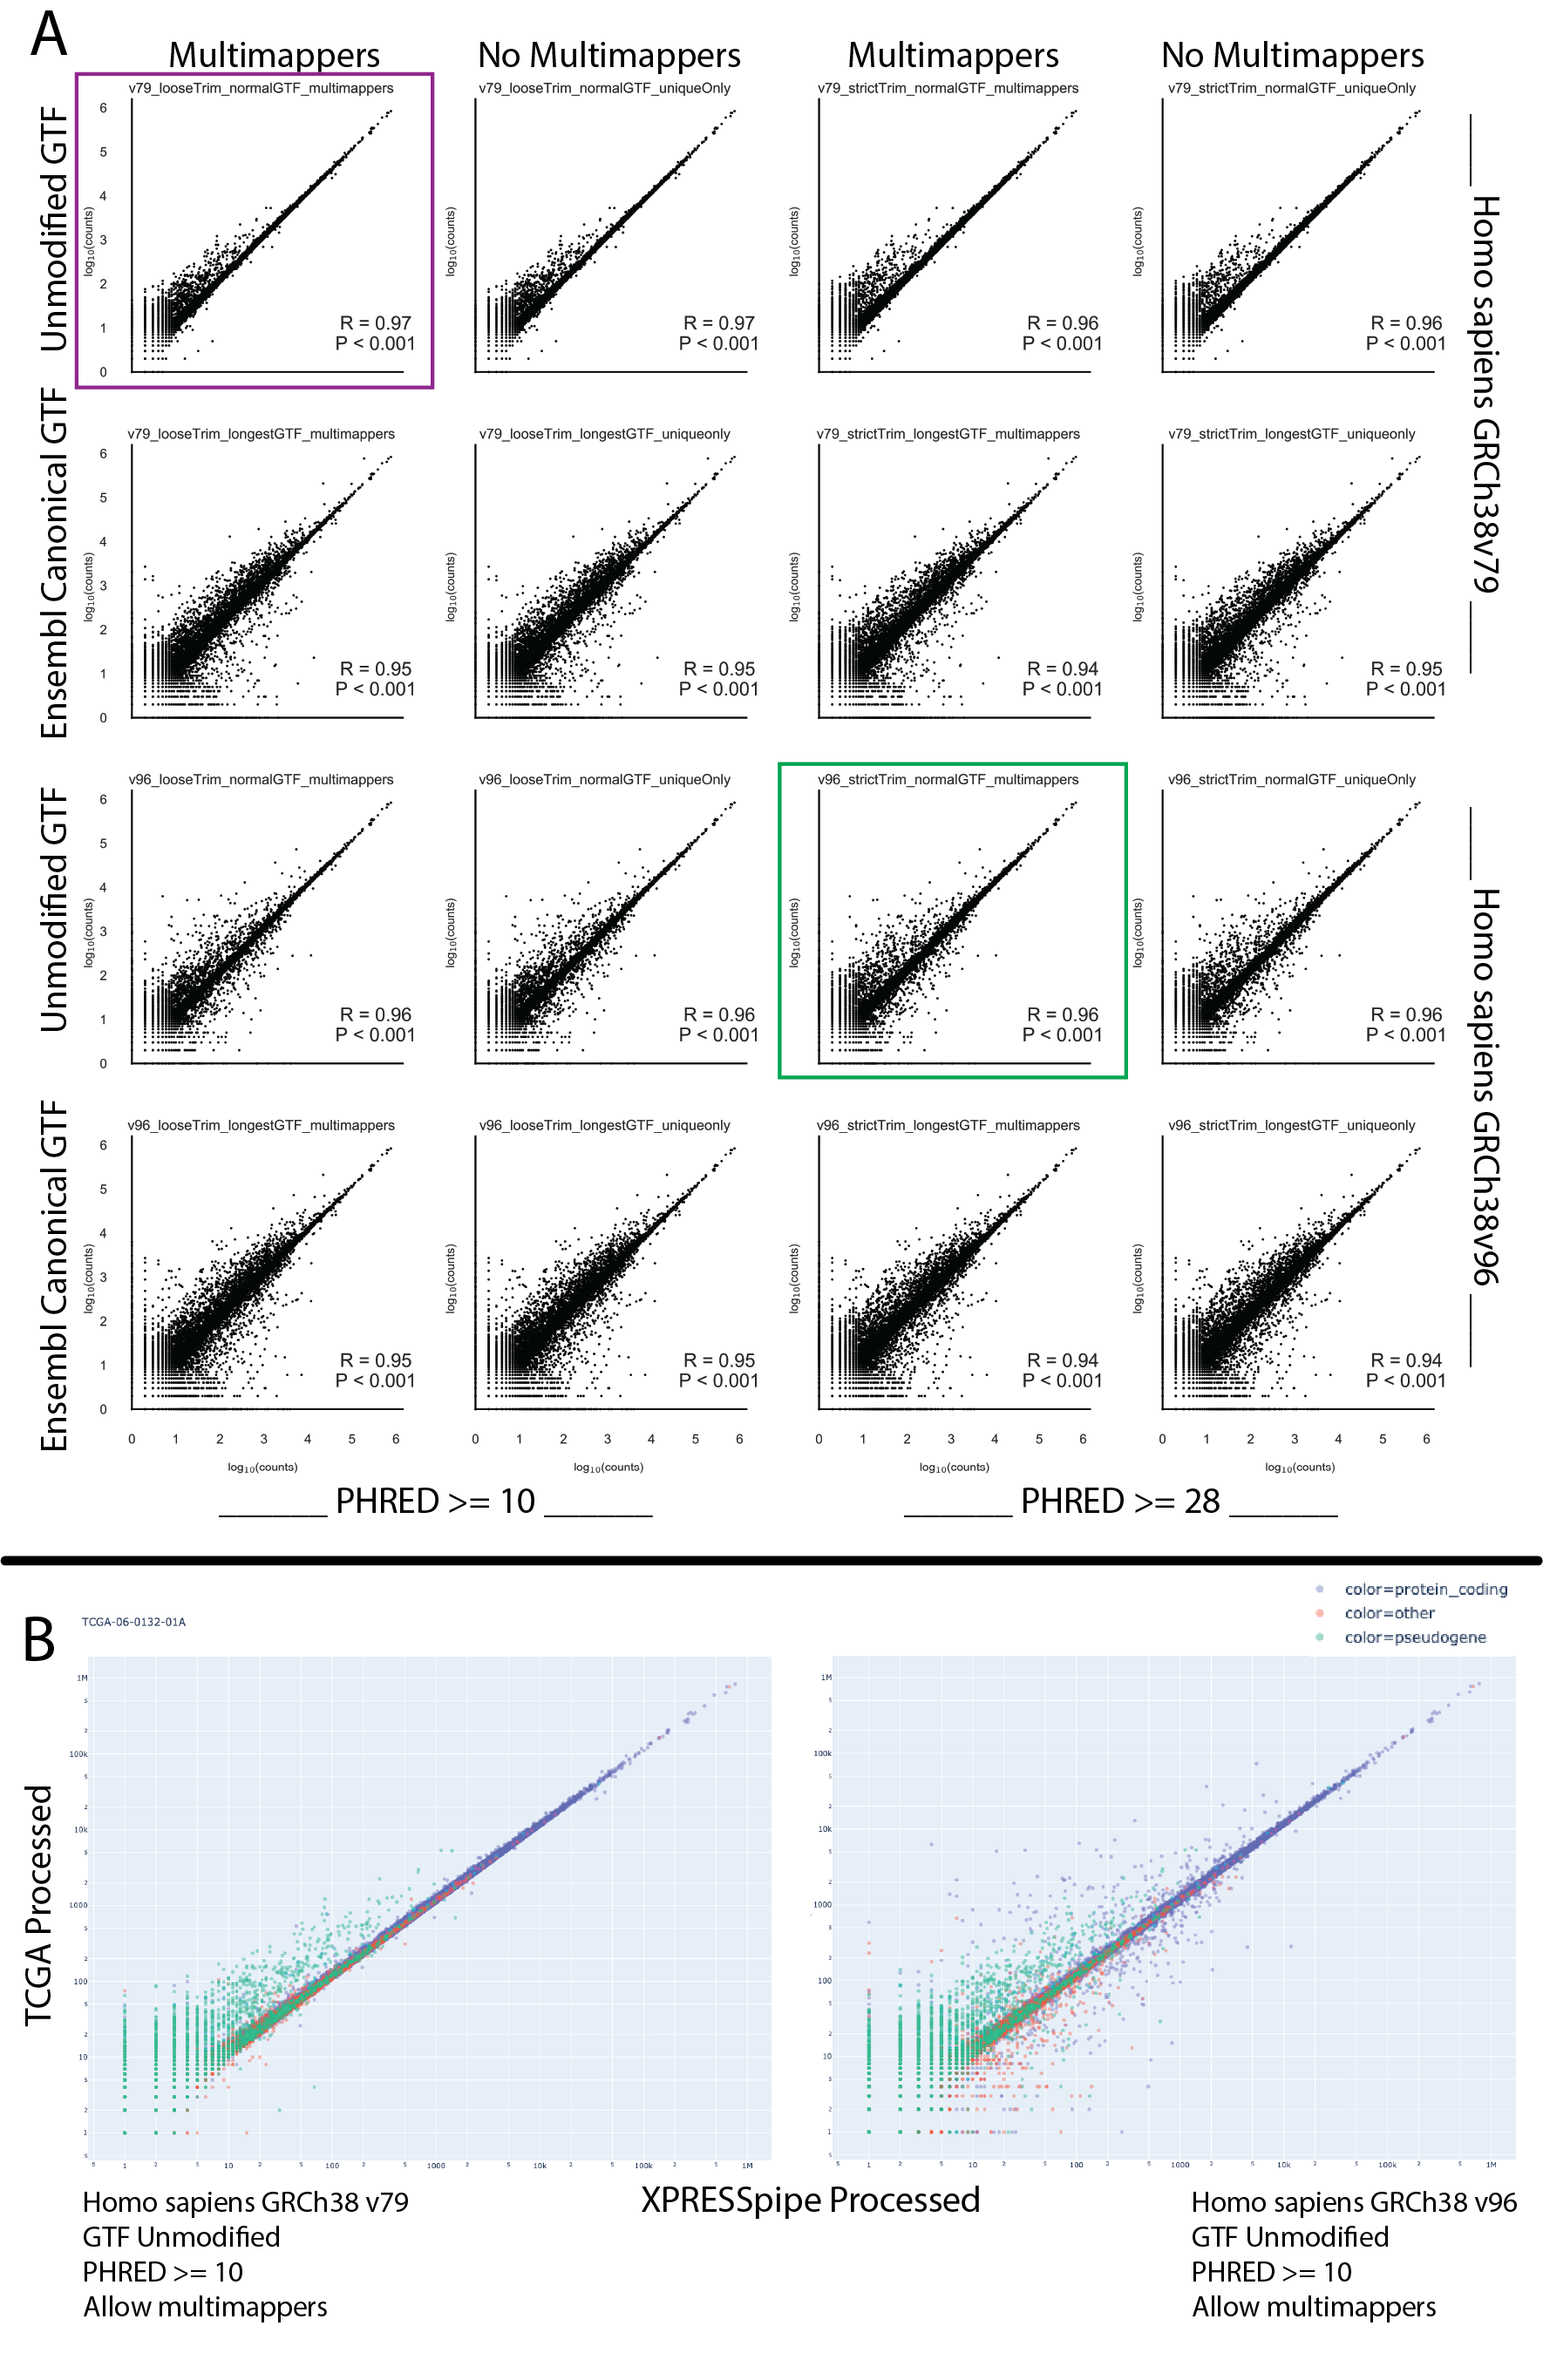
\includegraphics[width=180mm]{figures/xpresspipe_supplement4.png}
  \caption{Sample TCGA-06-0132-01A RNA-seq count data compared between TCGA count data and various conformations of the XPRESSpipe pipeline. A) An overview of how different conformations of the XPRESSpipe peRNAseq pipeline compared to the published TCGA count data. The x-axis data in the plot enclosed in maroon most closely mirrors the settings used in the published TCGA RNA-seq pipeline. The x-axis data in the plot enclosed in green used XPRESSpipe default settings and the most current reference transcriptome at time of writing. All points are log\textsubscript{10}(counts). B) An example of the differences arising solely by varying transcriptome reference version. The plot on the left was processed by using GRCh38v79 and the plot of the right was processed using CRCh38v96. Both used unmodified GTF files of the given file version, both allowed multimappers (however HTSeq does not use multimapped reads in quantification, so this does not effect the quantified reads in this case), and used a PHRED threshold greater than or equal to 10. Blue points represent protein coding genes, green points represent pseudogenes, and orange points represent other genes.}
  \label{fig:supplement4}
\end{figure}


\end{document}
